\documentclass[doc,natbib,floatsintext]{apa7}

\usepackage{multirow}
\usepackage{lscape}
\usepackage{amsmath}
\usepackage{amssymb}
\usepackage{subcaption}
\usepackage{hyperref}
\usepackage{microtype}
\usepackage{algorithm}
\usepackage{threeparttable} % allows notes in tables
\usepackage{algpseudocode}
\usepackage{setspace}
% \usepackage[toc,page]{appendix}
\usepackage{palatino}
\usepackage{graphicx}
\usepackage{tikz}
\usepackage{float}
\usepackage{lipsum}
\usepackage[american]{babel}
\usepackage{caption,placeins}
\usepackage{lineno}
\usepackage[title]{appendix}
% \usepackage[textsize=small]{todonotes}
\usepackage{silence}
\WarningFilter{latex}{Text page}
\WarningFilter{latex}{Float too large}



\hypersetup{colorlinks,linkcolor={blue},citecolor={blue},urlcolor={black}}
\usepackage{soul}
\definecolor{mygray}{gray}{0.6}
\usepackage{csquotes}
\usepackage[natbibapa]{apacite} 
\bibliographystyle{apacite}

\newenvironment{shade}{\color[rgb]{(191,191,191)}}{} %green 

% TODO NOTES JP
\definecolor{amber}{rgb}{1.0, 0.75, 0.0}
% \newcommand{\jptodo}[2][]{\todo[caption={\textbf{JPF}}, size=\scriptsize, color = amber, #1]{#2}~}
\newcommand{\jptodo}[2][]{\vspace{0.1cm} \hfil \todo[caption={\textbf{JPF}}, size=\footnotesize, color = amber, inline, #1]{#2}}

\newcommand{\todoN}[1]{\todo[inline]{New Sectione: #1}}

\newcommand{\xx}{\mathcal{X}} %Set of models
\newcommand{\dr}{D_{\mathrm{rev.}}}%{d_{\mathrm{new}}}%
\newcommand{\di}{D_{\mathrm{init.}}}%{d_{\mathrm{old}}}%
\newcommand{\hr}{h_{\mathrm{rev.}}}
\newcommand{\hi}{h_{\mathrm{init.}}}

\newcommand{\MYhref}[3][blue]{\href{#2}{\color{#1}{#3}}}

\newcommand\notesize{\fontsize{8pt}{9pt}\selectfont}



\title{Algorithms of Adaptation in Inductive Inference}
\shorttitle{Adaptation in Inductive Inference}

\author{Jan-Philipp Fränken$^{1}$, Nikos C. Theodoropoulos$^{1,2}$, and Neil R. Bramley$^1$}
\affiliation{$^1$ Department of Psychology, University of Edinburgh \\
            $^2$ Laboratory of Experimental Psychology, Suor Orsola Benincasa University of Naples}

\leftheader{Fränken, Theodoropoulos, and Bramley}

\abstract{We investigate the idea that human concept inference utilizes local adaptive search within a compositional mental theory space. To explore this, we study human judgments in a challenging task that involves actively gathering evidence about a symbolic rule governing the behavior of a simulated environment. Participants learn by performing mini-experiments before making generalizations and explicit guesses about a hidden rule. They then collect additional evidence themselves (Experiment 1) or observe evidence gathered by someone else (Experiment 2) before revising their own generalizations and guesses. In each case, we focus on the relationship between participants' \emph{initial} and \emph{revised} guesses about the hidden rule concept. We find an order effect whereby revised guesses are anchored to idiosyncratic elements of the earlier guess. To explain this pattern, we develop a family of process accounts that combine program induction ideas with local (MCMC-like) adaptation mechanisms. A particularly local variant of this adaptive account captures participants' hypothesis revisions better than a range of alternative explanations. 
We take this as suggestive that people deal with the inherent complexity of concept inference partly through use of local adaptive search in a latent compositional theory space.
}


\keywords{concept learning, program induction, language of thought, adaptive search, Markov chain Monte Carlo}


\authornote{Correspondence concerning this article should be addressed to: Jan-Philipp Fränken, Department of Psychology, School of Philosophy, Psychology and Language Sciences, University of Edinburgh, 7 George Square, EH8 9JZ, Scotland.  E-mail: \MYhref{mailto:janphilipp.franken@gmail.com}{janphilipp.franken@gmail.com.}
\addORCIDlink{Jan-Philipp Fränken}{0000-0001-5467-1887} 
\addORCIDlink{Nikoloas C. Theodoropoulos}{0000-0002-5454-261X}
\addORCIDlink{Neil R. Bramley}{0000-0002-4141-8476}}


\begin{document}
\setlength{\parindent}{2em}
\maketitle



\section{Introduction}
One of the defining aspects of being human is the ability to flexibly generate and adapt ideas and hypotheses. For example, we readily come up with possible faults if our car breaks down, or plausible maladies when we feel unwell, and we will readily refine and update these hypotheses as we gather more evidence. Our ideas often combine familiar objects, concepts, and relations, making them symbolic, amenable to communication but also to decomposition and piecewise adaptation. As a lighthearted example, suppose you are a detective trying to solve a murder at an old country house. Muddy footprints leading from the back door to the body might initially make you suspect the gardener. However, if your subsequent investigation reveals the gardener has an alibi, this may lead you to consider who else could be the wearer of the muddy boots. Perhaps it was the butler, whose shoes appear suspiciously newly polished. Next, supposing your assistant (pursuing their own line of reasoning) discovers some muddy boots hidden in the attic. This may make you reason that the murderer made the tracks deliberately to misdirect suspicion. Combining you assistant's evidence with your own observations, you can piece together the true order of events, in which the butler \emph{and} gardener conspired to kill their boss. One way to describe the detective's cognition in this toy scenario is as generating and dismissing a procession of independent explanatory hypotheses. However, another intuitive explanation is that it involves a process of sequential refinement or adaptation of a focal working hypothesis as different forms of evidence arrive. The muddy tracks are indeed part of the story, but further investigation reveals their relationship with the murder to be indirect, and the final hypothesis is arrived at after a sequence of revisions and edits. 

Symbolic concept induction can be framed, at the computational level \citep{marrfreeman}, as a top-down Bayesian inference over an infinite latent compositional theory space \citep{goodman2008rational, piantadosi2016logical,  bramley2018grounding}. At the heart of these approaches is the idea that the mind leverages a ``probabilistic language of thought'' --- roughly a system of conceptual primitives and stochastic rules for how they can be combined. Such models capture the fact that human creative hypothesis generation appears to exhibit ``infinite use of finite means'', seemingly requiring that it is based in a system with language-like properties of systematicity and compositionality \citep{fodor1975language, lake2015human}.

In practice, fully normative inference in compositional theory spaces is almost always intractable. Compositional hypothesis spaces are notoriously thorny to work with \citep{ullman2012theory}, with approximation involving extensive sampling even when reasoning in ``small worlds'' \citep{savage1954foundations}. One na\"ive approach is to assume a learner starts with a sufficiently expressive generative concept grammar \citep{bramley2018grounding} and uses this to generate a large number of prior samples or ``candidate hypotheses'' that can then be weighted and filtered based on their fit to evidence. % using rejection sampling. 
Depending on the grammar's expressivity, this procedure might require generating very large numbers of samples to ensure sufficient coverage of the space. Provided the true hypothesis is among those generated, it will gradually stand out from the alternatives as evidence arrives. Here, previous work on rule-based concept learning has proposed a rule-plus-exception account (RULEX), characterizing human inferences as utilizing a cascade of search strategies, starting with exact search over simple rules and, if necessary, progressing to search over more complex rules or allowing for more exceptions until a termination condition is met \citep{nosofsky1994rule}.  However, this appears to be an inefficient and cognitively implausible approach in general. Sampling from a concept grammar expressive enough to cover all plausible hypotheses even for a narrow domain will rarely produce the ground truth by chance.% unless it is very simple. 

Alternatively, a more promising approach may be to use stochastic search to explore the posterior directly. As an approximation to Bayesian inference, one can use Markov Chain Monte Carlo (MCMC) to stochastically adapt a working hypothesis in light of an underlying concept grammar and the relevant evidence, so directly entertaining a chain of autocorrelated hypotheses with each step biased towards whatever local alternatives have the better combination of prior plausibility and fit to evidence. A sufficiently long chain of considered hypotheses will approximate the posterior distribution. This approach does not require a learner to have already generated their final hypothesis before seeing evidence, but does produce order effects and local minima in which a learner's current hypothesis constrains what new hypotheses they can --- or are likely to --- conceive of next.

While a variety of particle filtering, MCMC and hybrid approaches have been used to construct normative predictions in recent symbolic concept induction research \citep{goodman2008rational, piantadosi2016logical, yang2022one}, there is yet to be a systematic exploration of whether any of these approximation schemes provide a compelling process account of human adaptation. That is, whether any variants of these algorithms reproduce human patterns of successes and failures in online inductive inference settings. One of the most ubiquitous non-normative response patterns are order effects in which sequential judgments are dependent, typically anchored to one another and thus inheriting errors and biases \citep{hogarth1992order}. Recently, these have been held as indicative of stochastic cognitive search in quantity judgments \citep{lieder2018anchoring}, conditional probability judgments \citep{dasgupta2017hypotheses} and in causal structure inference \citep{bramley2017formalizing}. Thus, we see the MCMC-like search as a promising algorithmic candidate for understanding the adaptation of compositional hypotheses in cognition. 

The goal of the current work is to investigate whether there is support for the ``adaptation as MCMC-like search'' proposal in an experimental setting that mimics the problem of generating and refining scientific theories. We focus on how people update their beliefs given two different sources of evidence: (1) evidence collected actively by the learner in further investigating their hypothesis (Experiment 1) --- similar to the detective's own investigations in our earlier example and (2) evidence gathered by another learner (Experiment 2) --- analogous to the insights the detective draws from their assistant's observations. Self-generated evidence comes with both benefits and costs \citep{markant2014better}. The key benefit of self-directed learning is an ability to target one's own hypotheses and uncertainty, for instance performing tests designed to distinguish between possibilities that have occurred to you. For a fully normative learner, able to consider and weight all possibilities, this will generally supercharge learning \citep{markant2014better}. However, the potential costs of self-generated data stem from the limits of the learner's current ideas. To the extent that the learner fails to consider plausible alternatives (as is very likely in our task) they may also fail to generate tests that adequately challenge the hypotheses they have generated. This can lead to a learning trap \citep{rich2018limits,settles2009active}, where testing patterns driven by ruling between hypotheses considered by the learner limit their progress to discovering other hypotheses outside this set.

We will measure to what extent participants' self-generated tests suggest confirmatory testing of their initial hypothesis, and consider the consequences of these testing patterns in the degree of change between their initial and revised guesses, and between initial and final accuracy.

The rest of paper is organized as follows. First, we briefly review related models of concept learning and motivate the probabilistic language of thought framework used to model inductive symbolic inference as \textit{program induction}. We then summarize recent work proposing process-level accounts of learning in related settings to motivate our algorithmic hypothesis. We sketch the inductive learning task and introduce the formal modeling framework. We then report on two experiments that vary the kind of additional evidence participants receive between their initial and revised judgments. We first unpack judgment patterns descriptively and then analyze them through the lens of our modeling framework. We end by discussing limitations and avenues for future work.

\section{Background}

\subsection{Language of Thought}
The idea that some of the most characteristically human forms of reasoning are driven by a symbol-and-rule-based conceptual system --- a \textit{language of thought} (LOT) --- dates at least as far back as \cite{fodor1975language}. The key idea is that creative thought, imagination and problem solving often seem to require compositionality and systematicity analogous to that enabled by a system of symbols and rules for their combination -- that is, a language. For example, if we have a primitive concept of a  ``triangle'' and of the property ``blue'' we can then imagine the compound concept of a ``blue triangle'', and could do so without having experienced this combination directly. With just a few more conceptual primitives, including some basic operators allowing quantification and logic, it becomes possible to generate, imagine or entertain an arbitrarily large space of concepts -- i.e., to hypothesize that ``all blue triangles are larger than any red triangles'' and so forth. Despite the fact that these are the aspects of human intelligence that have proven hardest to synthesize, the original language of thought hypothesis fell out of favor along with much of so-called ``good old fashioned AI'' with the rise of probabilistic rational models and neural networks \citep{chater1990autonomy}. However, recent work has rehabilitated the LOT idea by marrying it with computational approaches to symbolic inference under uncertainty \citep{piantadosi2016four, yang2022one}. Specifically, the idea that higher level cognition uses a LOT has been combined with probabilistic context free grammars (PCFGs) to model how a cognizer might stochastically generate hypotheses that can cover an infinite latent hypothesis space. Roughly, a PCFG consists of a set of stochastic production rules that can be used to iteratively compose --- and potentially to \textit{adapt} --- hypotheses by (re)combining primitives. The set of production rules and their probabilities implicitly specify a probability distribution over the infinite space of possible hypotheses.

\subsection{Learning as Program Induction}
By combining LOT-like symbolic representations with a stochastic grammar for generating hypotheses or ``programs'', human learning can be framed as a form of \textit{program induction} \citep{chater2013programs, calvo2014architecture, lake2017building,romano2018bayesian, rothe2017question, piantadosi2016logical,bramley2018grounding,rule2018learning}. Program induction approaches model learning as a stochastic search over a space of potential symbolic program-like representations \citep{rule2020child}. Work by \cite{goodman2008rational} demonstrated the utility of program induction for modeling human learning, introducing a rational model of symbolic concept learning which provided a good description of adults' generalizations across a Boolean concept learning task. More recent extensions of this idea have demonstrated that symbolic programs combining observed features with first-order logic provide good coverage of human inferences about categories of geometric objects \citep{piantadosi2016logical}. In another paper, \cite{lake2015human} demonstrate that a model that combines symbolic representations of concepts with a Bayesian fitness criterion outperforms deep-learning benchmarks in a one-shot classification task involving handwritten characters from real and invented languages. Moreover, the model introduced by \cite{lake2015human} had the ability to generate novel examples that were indistinguishable from humans across several ``visual Turing tests''.    

In addition to accounting for people's inferences and generalizations, program induction approaches to number learning have provided insights into how children might abduct a general understanding of natural numbers via bootstrapping \citep{piantadosi2012bootstrapping}. Using bootstrapping to learn difficult concepts has also been explored in related work modeling people's acquisition of functional concepts such as sorting or summing lists of inputs from a program induction perspective \citep{rule2018learning}. Asking questions to actively resolve uncertainty is another important component of human intelligence. Here, work by \cite{rothe2017question} and \cite{wang2019modeling} leveraged program induction ideas to develop a probabilistic model of open-ended question generation about the positions of two-dimensional objects in an ambiguous game environment. The authors used program induction to characterise this as involving a search for high-information--low-complexity queries with respect to resolving uncertainty about object positions.

A common theme across the above examples is that program induction involves stochastic generation of alternatives which are evaluated against one another using some fitness criterion. At a computational level, the generation of hypotheses is traditionally conceived as fully top-down problem, meaning that new programs are generated from a prior and only then evaluated against environmental stimuli. In a recent paper \cite{bramley2018grounding} questioned whether fully top-down generation is a plausible cognitive account. Specifically, the authors compared a top-down Bayesian approach against a partially bottom-up, \textit{instance-driven generation} (IDG) procedure during which encountered environmental stimuli inspire and partly shape the generation of new alternatives. Though further work is needed to validate the IDG proposal, initial results supported the notion that people use a partly bottom-up and data-inspired mechanism for generating hypotheses. More recently, program induction has been proposed as a broad account of learning under the ``child as a hacker'' metaphor, which emphasizes the inevitable incompleteness of any one learner's coverage of the compositional space of possible world-models or theories, and evokes process-level considerations such as the learner's intrinsic motivation and curiosity as drivers for progress and discovery \citep{rule2020child}.

\subsection{Process Models}
Bayesian models have been successful at characterizing many of the computational problems faced by cognitive agents, and frequently also characterizing aggregate patterns of human judgments in domains including causal structure learning \citep{gopnik2004theory, griffiths2005structure, griffiths2009theory}, social learning \citep{feldmanhall2019resolving} and concept learning \citep{goodman2008rational,piantadosi2016logical}. An idealized Bayesian agent reasons about a hypothesis space \(H\) on the basis of  data \(D\) and
arrives at an updated (posterior) belief \(P(H\mid D)\) by computing the normalized product of their prior belief \(P(H)\) and the likelihood of each hypothesis of producing the data \(P(D\mid H\)):

\begin{equation}
    P(H\mid D) = \frac{P(D\mid H)P(H)}{\sum_{H^{'}}P(D\mid H^{'})P(H^{'})}.
\label{equ:equ_1_bayes}
\end{equation}
  
However, direct application of Bayes' theorem is frequently intractable in naturalistic settings, and while collective behavior often appears noisily normative, individual cognizers are much more fallible \citep{jones2011bayesian}. This means that solutions achieved by real agents must be approximate and the best they can do is to strike a balance between computational cost and accuracy. 
Process accounts attempt to model how cognition uses algorithmic approximations to deal with intractable problems under consideration of limited computational resources \citep{griffiths2012bridging, sanborn2010rational,van2019cognition}. This section summarizes relevant work on process models of inference under uncertainty. While machine learning research has developed a plethora of approaches to approximating inference under uncertainty, two major flavors are those that use sampling, and those that use variational approximations \citep{sanborn2017types}. In the current work we focus on the potential use of sample-based approximations in cognition, in particular particle-based approximations and Markov Chain Monte Carlo (MCMC) methods.

\subsubsection{Particle Approximations}
Particle filters are a class of Monte Carlo algorithm that can approximate Bayesian inference where data arrives sequentially. A particle can be thought of as a single candidate hypothesis from the probability distribution in question. Filtering (reweighting and resampling) ensembles of particles as new data becomes available allows for the collection of particles to approximate the Bayesian posterior \citep{sanborn2010rational}. Several particle based process accounts of behavioral data found that individual participants are best fit as maintaining only a few particles --- essentially a small set of current working hypotheses --- in associative learning \citep{daw2008pigeon}, categorization \citep{sanborn2010rational}, and binary decision making \citep{vul2014one}. Across these domains, particle accounts help explain the paradoxical tendency for aggregate response patterns to reflect Bayesian norms while individual judgments are noisy and diverse.

An extreme version of particle filtering relevant to the present paper is the proposal that a learner's current hypothesis can be represented by a single particle that is resampled from the posterior if it becomes \textit{inconsistent} with new data (and kept otherwise). This idea has been formalized as the ``Win--Stay, Lose--Sample'' (WSLS) algorithm \citep{bonawitz2014win}, and has been shown to provide good agreement when compared with the performance of adults and preschoolers in several causal learning tasks \citep{bonawitz2014win,bonawitz2014probabilistic}. Importantly, while WSLS provides a promising starting point for understanding human reasoning, it does not provide a recipe for resampling hypotheses in the case that the learner decides to reject their current hypothesis. We now consider recent work addressing the question of how human learners search for new hypotheses. In particular, we explore the idea that this may involve \textit{adapting} an existing hypothesis rather than constructing a new one from scratch.

\subsubsection{Adaptive Search}
To model sampling and adaptation of particles, we turn to algorithms for sequential local search. Such algorithms generate sequences of (usually autocorrelated) hypotheses via a simple stochastic transition mechanism that is easier to compute than generating a new proposal from scratch. Two prominent approaches are Markov Chain Monte Carlo (MCMC) and hill climbing. Hill climbing can be achieved by proposing changes at random and accepting them only if they improve the previous hypothesis. This is good for rapidly improving a hypothesis, but limits the search space meaning that, in multimodal spaces such as a compositional theory space, the learner will tend to to get stuck in a local optimum; better than any of the adjacent hypotheses but worse than the global optimum \citep{ullman2012theory}. Here, we are specifically interested in the idea that human hypothesis adaptation might work a little like MCMC sampling, where proposed changes are accepted stochastically even if they do not improve the hypothesis, allowing the learner to escape local optima but still arrive more often at higher probability hypotheses. Because, by design an MCMC chain's stationary distribution is equal to the true posterior distribution, MCMC sampling asymptotically approximates the true posterior avoiding the need to evaluate an intractable normalization constant \(P(D) = \sum_{H}P(H,D)\), and allowing a sufficiently long chain to end in an unbiased sample from the posterior. 

\subsubsection{MCMC-like Search and Anchoring}
The proposal that stochastic local search forms a core component of hypothesis learning has been explored by \cite{dasgupta2017hypotheses}, who modeled human estimation of environmental conditional probabilities (e.g., ``what is the probability that an image containing a table also contains a [chair/computer/curtain]'') as involving an MCMC-like search with a limited number of iterations. Thus, their model provides a computational rationale for a variety of known cognitive biases, including \textit{subadditivity} \citep{fox1998belief}, \textit{superadditivity} \citep{sloman2004typical} and \textit{anchoring and adjustment} effects \citep{hogarth1992order}. The idea that people's hypothesis inferences are anchored by their initial ideas and adjusted by subsequent adaptations of these has been investigated by \cite{lieder2018anchoring}. Specifically, \cite{lieder2018anchoring} explored the proposal that cognizers adjust quantitative estimates (e.g., about the arrival time of a bus) away from an arbitrary initial seed or anchor via an MCMC-like process. They find that participants' judgments' degree of dependence on the anchor is broadly resource rational in the sense of striking a good balance between computational cost and accuracy. 

In the present work, we build on the literature on MCMC-like search, focusing on the algorithmic mechanisms underlying potential adaptations to an anchor. We build on a recent process account of online causal structure learning \citep{bramley2017formalizing}. \cite{bramley2017formalizing} found support for the idea that people update their causal structure beliefs in a probabilistic setting in a local and incremental way, considering just a few local edits when surprising evidence arrives. Their account assumes participants hold just a single global causal structure hypothesis at any time point, rather than a distribution over the full hypothesis space. Belief updates were modeled as involving very short MCMC Gibbs sampling chains where each new proposal might add, remove, or re-orientate a single causal connection in the light of the most recent data and conditional on the rest of the current hypothesis. In this way, the new hypotheses learners arrived at were those that accounted for the latest evidence they had seen while remaining anchored to their previous judgment. The previous judgment thus acted as a stand in for a prior in the absence of complete memory for the older data making the model a kind of ``single particle, particle filter''. This account outperformed a noisily normative account, WSLS, and a number of heuristic alternatives in capturing participants' judgment patterns. The best fitting parameters were consistent with adaptive search chains of just a few steps, with search behavior falling somewhere between MCMC and hill climbing. In the present work we extend this framework, taking it from the large but finite hypothesis space of possible causal graphs to the formally infinite space of possible concepts expressible in a LOT.  

\subsection{Search and Positive Testing}
Our secondary objective is to examine our process account under consideration of different forms of additional evidence. Specifically, we considered two forms of evidence: (1) additional evidence gathered by the learner and (2) evidence gathered by another learner. Evidence gathered actively via a learner's own directed actions \citep{settles2009active, gureckis2012self} is one of the most fundamental forms of data in individual cognition. In principle, well chosen actions or ``experiments'' performed by an active learner can improve their learning efficiency relative to passive observation because they can target areas of subjective uncertainty \citep{steyvers2003inferring, bramley2015conservative}. However, they can create pitfalls and learning traps given the bounded nature of our cognition \citep{rich2018limits}. For example, active learning without consideration of the full hypothesis space is likely to result in confirmatory testing biases in which a learner performs new experiments that seek to demonstrate the behavior predicted by their favored working hypothesis but that fail to distinguish it from possible alternatives that the learner has not considered \citep{klayman1987confirmation, wason1960failure}.

\section{Task}

\begin{figure*}[!th]
    \centering
    \begin{tikzpicture}
    \node[anchor=south west,inner sep=0] at (0,0) {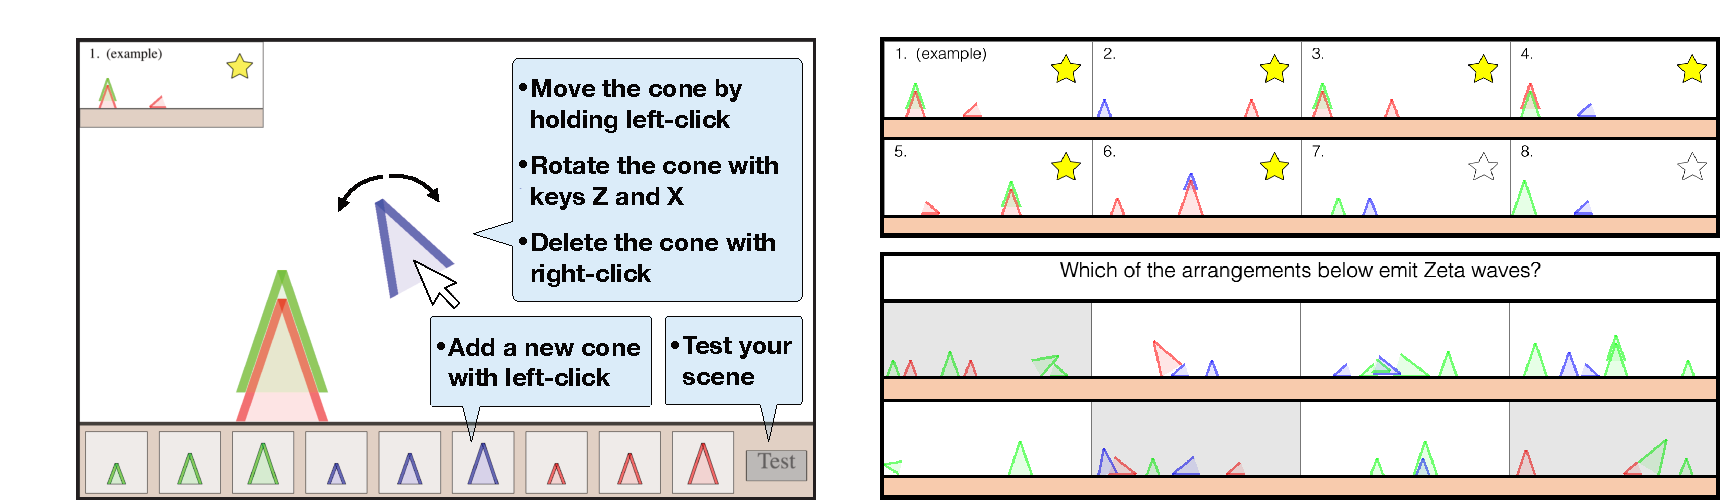
\includegraphics[width=.9\textwidth]{img/fig_1_zendo.pdf}};
    \draw (0.4,4) node[below] {\textbf{$\mathsf{a)}$}};
    \draw (6.8,4) node[below] {\textbf{$\mathsf{b)}$}};
    \draw (6.8,2.28) node[below] {\textbf{$\mathsf{c)}$}};
    \end{tikzpicture}
    \caption{Overview of the inductive learning task. a) Interface for generating and testing arrangements of cones including initial positive example. Star at the top-right indicates category membership (yellow fill = arrangement follows hidden rule). b) Example sequence of 7 tests generated by a learner using interface shown in a). The first example test was provided to all participants. c) Generalization phase: Participants decided which of a set of new scenes are rule following by clicking on them (grey background = selection). Hidden rule in the above example is $\exists(\lambda x_{1}: \text{ =}(x_1, red, color),\xx)$ (``there is a red cone'').}
    \label{fig:fig_1_zendo}
\end{figure*}

We adapt an environment introduced by \cite{bramley2018grounding} in which participants perform experiments to  discover a hidden rule hypothesis. The environment involves a two-dimensional box in which learners can place and arrange triangular objects called ``cones'' of a range of colors and sizes (Figure~\ref{fig:fig_1_zendo}a). Objects in the environment are governed by realistic simulated physical laws and certain combinations and arrangements of objects produce a causal effect when tested. A star shape at the top-right with yellow fill indicates category membership (i.e., whether the arrangement follows the hidden rule / produces the causal effect). The learner's goal is to infer the hidden rule that determines the circumstances under which the effect occurs. For example, if the true rule is that ``there is a small red cone'' any scene that includes a small red cone will produce the causal effect. We probe learning by asking and incentivizing learners to (1) generalize by labelling a set of novel scenes as rule following or not (Figure~\ref{fig:fig_1_zendo}c) and (2) provide an explicit written guess of the unknown rule concept. In our experiments, we will probe participants' learning twice: first after a they complete an initial active learning phase in which they gather evidence $\di$, and again after completion of a second learning phase in which they either gather additional evidence $\dr$ themselves or observe additional evidence gathered by another learner (Figure~\ref{fig:fig_2_experiments}; see Methods for details).

\subsection{The Grammar}
There are any number of possible grammars and choices of primitives capable of expressing the rules we explore in this task. However, following \cite{piantadosi2016logical}, we adopt an expressive grammar that combines the basic object features of size \(\in\{\text{small, medium, large}\}\), color\(\in\{\text{red, blue, green}\}\), orientation\(\in\{\text{up, down, left, right}\}\) and grounded\(\in\{\text{yes, no}\}\) with first order (predicate) logic and use lambda abstraction \citep{church1932set} to bind assertions to one or multiple variables. Table \ref{table:table_1_primitives} contains the full grammar. Continuing the example above, we can express ``there is a small red cone'' as $\exists(\lambda x_{1}\!:\! \land(\text{=}(x_1, small, size), \text{=}(x_1, red, color)),\xx)$ which can be read as ``there exists a cone (or element) $x_1$ in the set of all cones in a rule-following scene $X$, such that $x_1$ has the size small and color red''. Arbitrarily complex hypotheses can be constructed by binding more than one variable. For example, ``the largest cone is red'' can be expressed as $\exists(\lambda\!x_1\!:\forall(\lambda\!x_2\!:\land(\text{=} (x_1, red, color), > (x_1,  x_2, size)), \xx), \xx)$. Pragmatically, we also include a relational primitive of ``contact'' that can hold between any pairs of cones. We will use our grammar to translate participants' explicit written guesses of the unknown rule concept into lambda abstraction representations used for formal analysis. 


\begin{figure*}[t]
    \centering
    \includegraphics[width=.9\textwidth]{img/fig_2_experiments.pdf}
    \caption{Illustration of our experimental setup. In both experiments, learners first gather initial evidence ($\di$) using the interface shown in Figure~\ref{fig:fig_1_zendo}a. They then make initial generalizations (grey background = selection) and provide an initial explicit rule guess. In Experiment 1, learners then collect additional evidence ($\dr$) themselves and are invited to revise their generalizations and explicit rule guesses if they wish. The true hidden rule is the same across both learning phases. In Experiment 2, learners were recruited in pairs. The initial learning phase including initial generalizations and explicit rule guesses was identical to Experiment 1. In the second learning phase, participants were shown the initial evidence collected by the other learner (facing the same hidden rule) alongside their own, before being invited to revise their generalizations and guesses.
    }
    \label{fig:fig_2_experiments}
\end{figure*}


\begin{table}[ht]
\caption{Concept Grammar.}
\small
\begin{center}
\resizebox{\columnwidth}{!}{\begin{tabular}{lc}
\toprule
There exists an object $x_i$ such that... & $\exists(\lambda\!x_i\!:,\xx)$ \\
For all $x_i$ ... & $\forall(\lambda\!x_i\!:,\xx)$\\
There exist(s) \{at least, at most, exactly\} $N$ objects $x_i$ such that... & $N_{\{<,>,=\}}(\lambda\!x_i\!:, N,\xx)$\\
Feature $f$ of $x_i$ has value \{larger, smaller, (or) equal\}  to $v$ & $\{<,>,\leq,\geq,=\}(x_i, v, f)$\\
Feature $f$ of $x_i$ is \{larger, smaller, (or) equal\} to feature $f$ of $x_j$  & $\{<,>,\leq,\geq,=\}(x_i, x_j, f)$\\
Relation $r$ between $x_i$ and $x_j$ holds & $\Gamma(x_i, x_j, r)$ \\
Booleans \{and,or,not\} & $\{\land,\lor,\neq\}(x)$\\
\bottomrule
\end{tabular}}

\label{table:table_1_primitives}
\raggedright {\notesize Note that $\{<,>,\geq,\leq\}$ comparisons only apply to the feature size}.
\end{center}
\end{table}




\subsection{Production Rules}

\subsubsection{Sampling from the Prior}
To generate symbolic hypotheses relevant to our inductive problem --- that is, possible rules governing when the causal effect occurs --- we use a \emph{probabilistic production process} capable of producing all grammatical compositions of the primitives relevant for the learning setting. In practice, we simulate this production process by iteratively rewriting subparts of a string until a termination condition is reached \citep{manning1999foundations, goodman2008rational,piantadosi2016logical,bramley2018grounding} but are agnostic about how such a process could be implemented neurally (see Appendix~A-1 for technical details).


\subsubsection{Prior Probabilities}
By design, our production grammar embodies a prior preference for simplicity. That is, the production process will terminate in a short and simple hypothesis more frequently than more complex hypotheses. For example, there is a geometrically decreasing probability of generating hypotheses with a larger number of bound variables --- half of the hypotheses produced make reference to only a single subset of the objects in a scene $x_1$ (i.e., have only one quantifier), a quarter refer to two subsets $x_1$, $x_2$, 12.5\% to three subsets $x_1$, $x_2$, $x_3$, and so on. The prior probability of a given expression can be derived from the product of the probabilities of the sequence of productions that created it. This product inevitably decreases with the length of productions. Following the notation in \cite{goodman2008rational}, we write the prior generation probability for hypothesis \(h\) as:

\begin{equation}
    P(Deriv\textsubscript{h}\mid\mathcal{G},\tau) = \prod_{s\in \text{Deriv}_{h}} \tau(s)
\label{equ:equ_2_prior}
\end{equation} 

where \(\mathcal{G}\) refers to our grammar, \(\tau\) refers to the production probabilities, s \(\in\) \(Deriv\)\textsubscript{\(h\)} refers to the productions in the derivation, and \(\tau(s)\) to the probability of each production. While derivations can vary in length, each derivation ultimately arrives at a termination production at which no further productions are sampled (see Figure~\ref{fig:fig_3_adaptation}a and Table~\ref{table:table_a1_1_productions} for further details). One complicating detail is that there are typically multiple ways of realizing a given semantics in syntax. Consider again the concept ``there is a small red cone'' which can be written as $\exists(\lambda x_{1}\!:\! \land(\text{=}(x_1, small, size), \text{=}(x_1, red, color)),\xx)$. Though this rule is syntactically distinct from ``there is a red small cone'' --- $\exists(\lambda x_{1}\!:\! \land(\text{=}(x_1, red, color),\text{=}(x_1, small, size)),\xx)$, both expressions have the same meaning. That is, they will return the same truth value for any scene. The number of semantically equivalent expressions increases as an inverse function of the prior generation probability of a rule (essentially increasing with rule complexity, Equation~\ref{equ:equ_2_prior}). We thus derive a polynomial adjustment that we later use to approximate the total prior generation probability of a semantic rule class from the generation probability of a specific syntactic exemplar from that class (further details on prior generation probabilities are provided in Appendix~A-1 and A-2).

\begin{figure*}[!th]
    \begin{center}
    \begin{tikzpicture}
    \node[anchor=south west,inner sep=0] at (0,0) {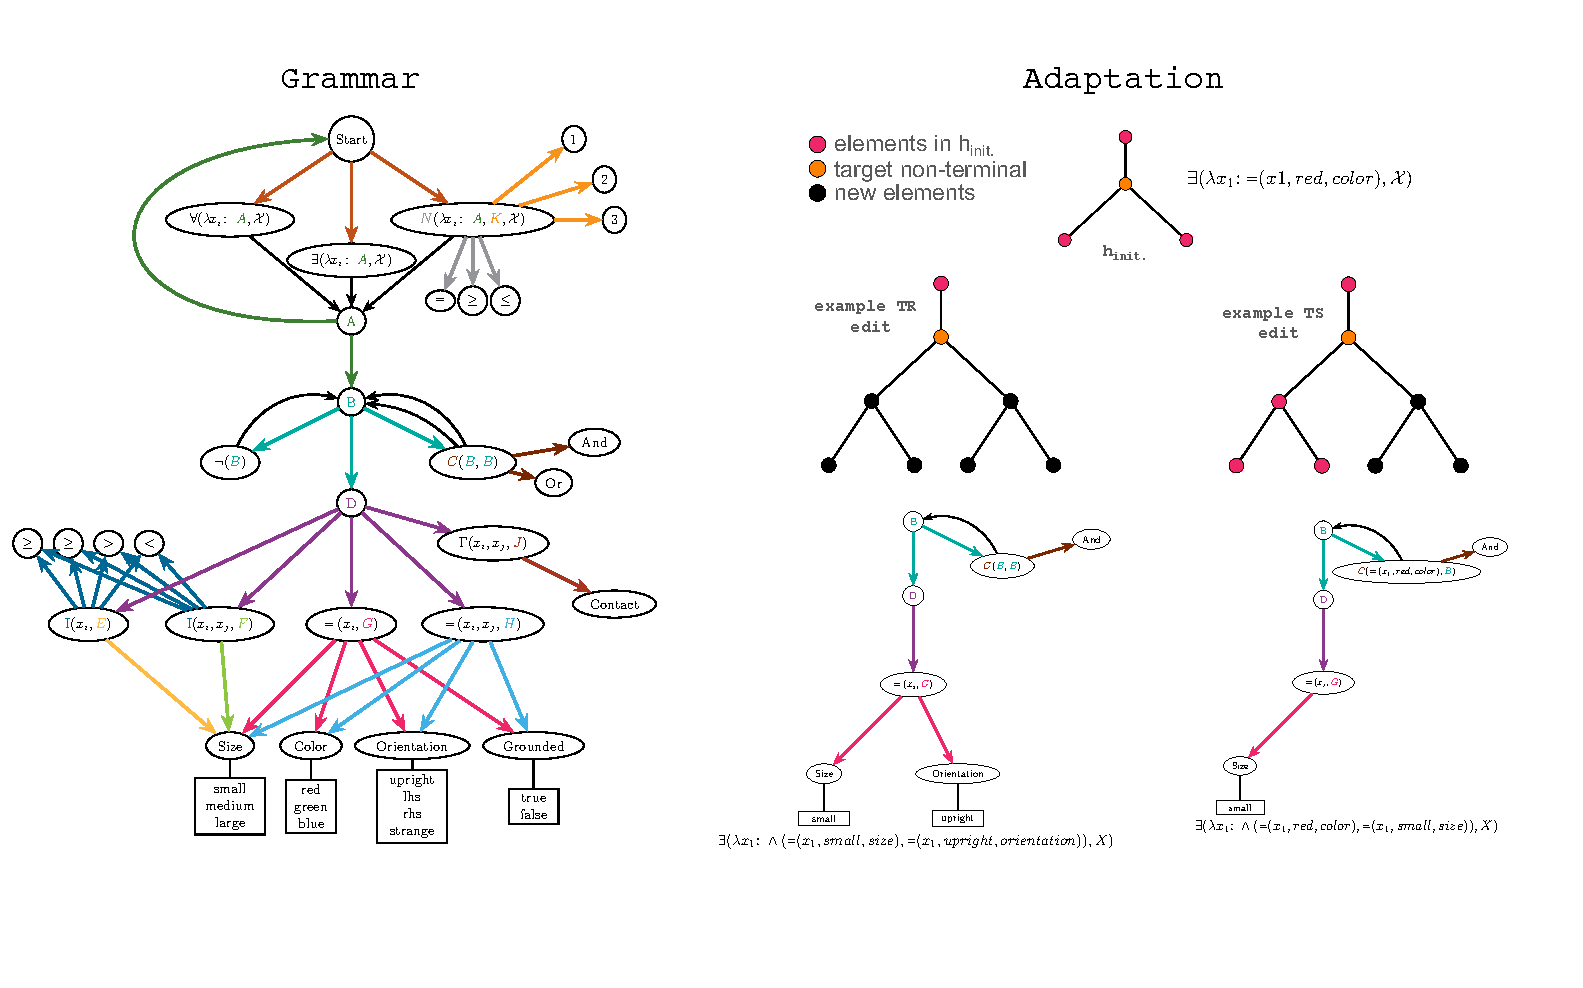
\includegraphics[width=.95\textwidth]{img/fig_3_adaptation.pdf}};
    \draw (0.5,8.9) node[below] {\textbf{$\mathsf{a)}$}};
    \draw (7,8.9) node[below] {\textbf{$\mathsf{b)}$}};
    \end{tikzpicture}
    \end{center}

    \caption{a) Visualization of the top down rule generation process using our concept grammar. A rule is generated by starting at ``Start'' and following outgoing edges stochastically, in each case replacing the non-terminal symbol (capital letter with color matching the arrow) with the string at the arrow's target. The process naturally terminates when no non-terminal symbols remain (see Table~\ref{table:table_a1_1_productions} for further details). b) Illustration of different adaptation mechanisms. Example rule $\hi$ $\exists(\lambda x_{1}\!:\! \text{ =}(x_1, red, color),\xx)$ (``there is a red cone''; top) and example ``Tree Regrowth'' (TR) and ``Tree Surgery'' (TS) adaptations (bottom; see main text and Appendix~A-1 and A-4 for further details). 
    }
    \label{fig:fig_3_adaptation}
\end{figure*}

\subsection{Likelihood}
We assume a simple likelihood function that allows for some stochasticity in the behaviour of each rule \citep[cf.][]{goodman2008rational,lewis2014error}, such that the likelihood that a hypothesized rule $h$ correctly labels a set of scenes $D$ is a decreasing exponential function of its number of mispredictions

\begin{equation}
    P(D\mid h, b) \propto e\textsuperscript{-b |F|}
\label{equ:equ_3_likelihood}
\end{equation}

where $F$ corresponds to the set of scenes predicted by the rule that do not match the true observed labels $T$: $F$ = \{\(d \in D \mid h(d) \ne T(d)\)\}. \(b\) is an inverse temperature parameter such that as \(b\to\infty\), the likelihood of a scene producing stars when the true rule says it will not, or not producing stars when the rule says it will, approaches zero.

\section{Models of Adaptation}
This section introduces the specific models of hypothesis adaptation we will compare to human inference patterns. We focus on predicting participants' revised explicit rule guesses $h_{rev.}$ which were elicited after participants collected both initial $\di$ and revised evidence $\dr$ (see Figure~\ref{fig:fig_2_experiments} and Methods). 

\subsection{Normative Simulations}
We first consider a practically unbounded Bayesian learner that functions as a normative benchmark for our model comparisons. This model approximates a posterior distribution over the hypothesis space at each phase of the experiments and marginalizes over this posterior to make generalizations and guesses as to the true hidden rule. The posterior over rules after seeing initial evidence $D = \{\di\}$ or a combination of initial and revised evidence $D = \{\di,\dr\}$ is given by:

\begin{align}
    P(H\mid D)\propto P(D\mid H)P(H)
\label{equ:equ_4_posterior}
\end{align}

and the marginal posterior probability that a newly observed scene $s$
is rule following (across all possible rules) corresponds to:

\begin{equation}
    P(s\mid D) = \sum_{h\in H}P(s\mid h)P(h\mid D).
\label{equ:equ_5_marginal_label_prob}
\end{equation}

In practice, these equations cannot be evaluated directly because $H$ is infinite. However, the intractable posterior $P(H\mid D)$ over rules and predictive distributions over selections for new scenes $P(s\mid D)$ can be approximated in various ways. Here, we use an MCMC chain with a ``Tree Regrowth'' proposal distribution \citep{goodman2008rational} to generate large posterior samples (see Appendix~A-3 for further details of this approximation scheme). For constructing normative predictions, we used sufficiently numerous and lengthy MCMC chains to erase the patterns of anchoring on the chain-seed, since these are integral to our process ideas. Thus, the normative learner predicts that participants' initial ($\hi$) and final rule judgments ($\hr$) are independent conditional on the evidence.

\subsection{Win--Stay, Lose--Sample}
We next consider an idealized manifestation of Win--stay, lose--sample \citep[WSLS,][]{bonawitz2014win}. Under WSLS, the learner samples their initial hypothesis $\hi$ from $P(H\mid \di)$. Then upon exposure to additional data $\dr$, WSLS keeps the current hypothesis with a probability tied to $\hi$'s ability to account for the new data, or else samples a new hypothesis. Concretely, the chance WSLS draws a new sample is the complement of the likelihood of the new data given the old hypotheses: 

\begin{equation}
    1 - P(\dr \mid \hi, b).
\label{equ:equ_6_wsls}
\end{equation}

This means that hypotheses which provide a good fit to the additional set of test scenes are likely to be kept (even if other hypotheses would also provide a good fit), and the worse the initial hypothesis does, the more likely the learner is to resample from the posterior distribution $P(H\mid \di,\dr)$ which here leverages the standard likelihood ratio comparison (see Equation~\ref{equ:equ_a3_1_mcmc} in Appendix~A-3). We note that this behavior predicts an all or none dependence on the initial hypothesis $\hi$: Either $\hr$ will be stay the same as $\hi$ with probability $P(\dr\mid \hi, b)$, or it will be an unbiased posterior sample $P(H\mid\di,\dr)$ with probability $1 - P(\dr\mid\hi,b)$. Though WSLS predicts an order effect in which the use of posterior distribution over revised hypotheses is conditioned on the fitness of $\hi$ to the new data, it is not \emph{yet} a candidate process model, because it provides no recipe for how a learner resamples in the cases they decide to do so. 

\subsection{Hypothesis Adaptation as Local Search}

Our central hypothesis is that people update their beliefs through incremental adaptation. This means that we do not expect just all-or-none dependence between a learner's $\hi$ (initial rule guess) and $\hr$ (revised rule guess). We rather expect a graded dependence reflecting some form of local (MCMC-like) search for promising alternatives \citep{bramley2017formalizing}. We now introduce two process models under which adaptation is modeled as a limited local MCMC search for alternatives under consideration of the full evidence $D = \{\di,\dr\}$ available to a learner after completion of the revised learning phase of our task. The first process model uses the established proposal distribution used for rule search, known as ``subtree-regeneration'' or ``Tree Regrowth'' \citep{goodman2008rational}. The second process model uses a novel, and more local variant, that we name ``Tree Surgery'' (for details see Figure~\ref{fig:fig_3_adaptation}b and Appendix~A-4). We nest the two proposals within the WSLS framework, meaning that $\hr$ will be identical to $\hi$ with probability $(\dr\mid \hi,b)$, or it will be a \textit{local adaptation} of $\hi$ obtained by the respective local search procedure with probability $1 - P(\dr \mid \hi, b)$. The local search procedures implemented by our process models differ from WSLS in terms of their mechanistic implementation of editing hypotheses when the initial rule guess proves sufficiently inconsistent with new evidence to motivate a change. While WSLS resamples a new hypothesis from scratch, our process accounts \textit{adapt} the initial hypothesis \(\hi\). In other words, the generation of new proposals is conditioned on a learner's initial guess \(\hi\) and the data $D$ = $\{\hi,\hr\}$. As such, adaptation is modeled by stochastic transitions from \(\hi\) to \(\hr\) involving a short sequence of edits, potentially reflecting an anchoring process in which the initial hypothesis acts as a stand in for a prior \citep{bramley2017formalizing}. 


\subsubsection{Tree Regrowth (TR-Learner)}
Our first process learner implements edits to an existing hypothesis \(\hi\) by regrowing random subtrees from the overall hypothesis tree structure. Tree Regrowth (TR) works by sampling a random %non-terminal component 
node or edge of the original hypothesis and regrowing a new subtree below. Figure~\ref{fig:fig_3_adaptation}b illustrates one potential step of a TR process, targeting the edge between $\exists$ and $=$, resulting in the new rule $\exists(\lambda x_{1}\!:\! \land(\text{=}(x_1, small, size), \text{=}(x_1, upright, orientation)),\xx) $ --- ``there exists a small cone that is oriented upright''. Here, the TR-Learner essentially replaces $\text{=}(x_1, red, color)$ with $B$ and runs the grammar until termination (Figure~\ref{fig:fig_3_adaptation}a). Diverging from idealized WSLS and normative simulations, we assume a TR-Learner uses only a few \(k\) regrowth steps to adapt their prior hypothesis without losing it altogether. Following \cite{bramley2017formalizing}, we model a learner's variability in ``search length'' \(k\) on a given trial (i.e., the length of the MCMC chain) by sampling $k$ from a shifted Poisson distribution with an average search length of $\lambda + 1$:

\begin{equation}
    P(K=k\mid\lambda) =\sum_{0}^{\infty}\frac{\lambda^{k_{i}}e^{-\lambda}}{k_{i}!} + 1.
\label{equ:equ_7_poisson}
\end{equation}

Considering an initial hypothesis \(\hi\) and evidence  \(D=\{\di,\dr\}\), the TR-Learner adapts an initial rule $k$ times, starting with $h_{0}$ = $\hi$ and ending with $h_{k}$ = $\hr$, where each $h_{i+1}$ is generated by an MCMC step. As such, a tree can be modified up to $k$ times, depending on how often a new modification was accepted by means of Equation~\ref{equ:equ_a3_1_mcmc}.

\subsubsection{Tree Surgery (TS-Learner)}
While Tree Regrowth is a convenient form of MCMC for machine learning applications, due to its reuse of the general PCFG hypothesis generation mechanism, it is less clear whether it would be a good candidate adaptation mechanism for cognition. Tree Regrowth tends to produce hypotheses that differ substantially from their predecessors. The higher up the tree each regrowth process is initiated, the more of the original tree is overwritten. Indeed, each update overwrites an average of half of the tree, and within a few steps the updated hypothesis is likely to bear little resemblance to the starting point, typically retaining only its top level quantification but changing what features and assertions they pertain to. Intuitively, human hypothesis adaptation is often considerably more ``surgical'' than this. For instance, it seems natural that adaptations to the hypothesis shown in Figure~\ref{fig:fig_3_adaptation}b might result in a more specific hypothesis such as that there needs to be a small red cone. This kind of change amounts to introducing a branch conjunctively to the hypothesis while \emph{retaining} its descendants. Alternatively, a proposal might remove a part of a more complex rule. For example, if one started with the rule ``there is a red lying on its left hand side'' and new evidence revealed that an upward standing red cone is rule following, one might then simplify the rule to ``there is a red'' assuming that color is the only relevant feature. An even simpler surgical edit to a rule could be to replace one boolean with another (i.e., replace an $\land$ with an $\lor$). This might be appropriate when new evidence suggests that being ``red'' and ``lying on its left hand side'' are individually sufficient features. In addition to targeting Booleans, we assume TS edits can also involve simple replacements of quantifiers with no change in the predicate or scope. For example, the rule ``there is a small'' --- \(\exists(\lambda x_{1}\!:\! \text{=}(x_{1},small,size), X)\) --- might simply be adapted to become ``all are small'' $\forall(\lambda x_{1}\!:\! \text{=}(x_{1}, small,size),X)$ or ``there is exactly one small'' $N(\lambda x_{1}\!:\! \text{=}(x_{1}, small,size),1, X)$ (see Appendix~A-4 for further technical details).

As with the TR-Learner, our Tree Surgery account adapts \(\hi\) by proposing \(k\) edits under consideration of  \(D=\{\di,\dr\}\) and asymptotically produces a new sample hypothesis from the posterior. The difference between the TR-Learner and TS-Learner is in the locality of proposed edits. The TS-Learner implements ``surgical'' local proposals while keeping the rest of the tree fixed as far as possible. The set of possible replacements for a given node are those that maintain compatibility with the type signatures of the components above and below in the tree. We note that both methods generate new proposals in a a top-down fashion, meaning that novel adaptations are suggested at random and not inspired by particular observations but their acceptance probability is shaped by their relative fit to the evidence. An example of bottom-up data-driven search has been explored by \cite{bramley2018grounding}.

\subsubsection{Alternative Accounts}
To assess how competitive our adaptation proposal is, we pit it against the rules-plus-exception (RULEX) model \citep{nosofsky1994rule}. RULEX has been used to model human learning in a number of concept learning studies, including classic experimental results by \cite{medin1978context}. RULEX works by applying a cascade of increasingly complex and approximate search procedures as required, to arrive at a symbolic rule. Traditionally it has been used in a propositional ``Boolean logic'' setting where rules do not require bound variables, but we here extend it to handle our setting. In brief, RULEX begins by searching for a rule referring to a single feature (exact search). If exact search succeeds, meaning that a rule is generated that correctly classifies all data points, RULEX adopts that rule permanently and terminates. Otherwise, RULEX continues by either performing an imperfect search over simple rules or a new exact search over conjunctive rules (i.e., rules pertaining to two features combined with a Boolean). For the imperfect search it again terminates if this search succeeds, where the success criterion is now that a rule is found that makes less than a threshold number of misclassifications. If the conjunctive search succeeds it terminates and adopts the conjunctive rule. 
If imperfect or conjunctive search fails (i.e., too many incorrect classifications), RULEX switches to the other type of search \citep[for details, see][]{nosofsky1994rule}. Finally, if both fail, RULEX searches for an imperfect simple or conjunctive rule, lowering its theshhold for termination to allow for more and more misclassifications (i.e., ``exceptions'') until a rule is found that passes the bar. Misclassifications are finally added to the final rule as listed disjunctive ``exceptions''

RULEX does not work ``out of the box'' on our task because our setting requires predicate logic and further involves disjunctive as well as conjunctive rules (see Table~\ref{table:table_2_rules}). That is, rules involve quantifications like ``all'' and ``there exists'' and can refer to multiple subsets of objects in the environment potentially combining several conjunctions, disjunctions and negations. To accommodate this larger possibility space, we had our implementation of RULEX search over rules sampled from our hypothesis space constrained to either simple rules (no conjunctions or disjunctions but allowing arbitrary quantification and negation) or conjunctive and disjunctive rules (those containing exactly one conjunction or one disjunction again allowing for arbitrary quantification and negation). Just as with our other process models, we assume RULEX's ability to search is limited. Therefore, we assume that a RULEX learner considers a finite number of hypotheses sampled from an appropriately restricted prior at each stage, with the number sampled from a shifted Poisson distribution just as with our other process models (Equation~\ref{equ:equ_7_poisson}). We provide further details our our implementation of RULEX in the Model Comparison section and Appendix~A-5. 

\section{Overview of Experiments}
We study human learning across two experiments. For each experiment, our primary analysis compares participants' generalizations and explicit rule guesses against those of a large posterior sample. We then investigate quantitatively which of our competing process accounts is best at finding participants' revised rule guesses $\hr$. To foreshadow, our model comparison finds support for several of these models but best supports the idea that participants' revised rule guesses $\hr$ are best predicted by means of a local, TS-like adaptation to their initial rule guesses $\hi$.

\section{Experiment 1}
\subsection{Methods}
\subsubsection{Participants}
Ninety Participants (age 36.8$\pm$10.5 years [M$\pm$SD]) were recruited from Amazon's Mechanical Turk (hit approval rate $\geq$ 95\%) and paid \$4.50 upon completion + [\$0.05,\$2.00] bonus based on the accuracy of their revised generalizations. We were able to translate 248 of the total 450 free responses (each trial included two explicit rule guesses, one initial guess, and one revised guess) into our grammar.\footnote{The other free responses were either ambiguous (e.g., ``I saw this one had cones inside the other and there was one more cone in this group'', $N$ = 92) or nonsensical (e.g., ``very nice task'', $N$ = 110).} We thus use all 450 trials for our primary analyses but only the 248 trials with unambiguous initial and revised rule guesses during quantitative model comparisons.

\subsubsection{Software}
Both experiments were implemented using a javascript port of the {\tt Box2D} physics game engine and ran in participants' browsers. Scenes were displayed and constructed using an interactive 800 by 500 pixel iframe window embedded in the full screen task interface. A demo version of Experiment 1 is available \MYhref{https://zendo-cond-3.herokuapp.com/}{here}.


\subsubsection{Cover Story}
Following \citep{bramley2018grounding}, we used a minimal ``alien planet'' cover story to frame the task in both Experiments. In it, participants act as space scientists tasked with working out the laws (rules) governing why particular combinations of alien objects (``cones'') produce alien forms of radiation. The instruction phase included five examples of already discovered radiation (shown in Figure~\ref{fig:fig_4_test_rules}) which served to orientate participants to the relevant features of the scenes. 

\begin{figure}[!th]
    \begin{center}
      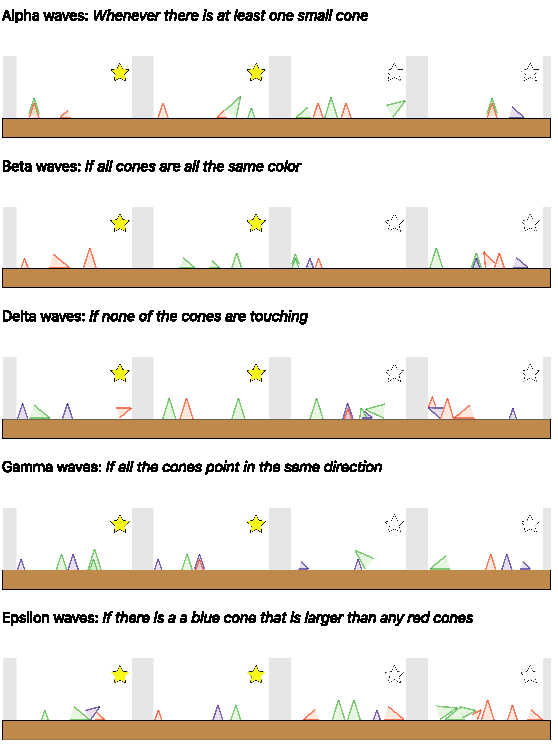
\includegraphics[width=0.4\columnwidth]{img/fig_4_test_rules.pdf}
    \end{center}

    \caption{Example causes of radiation as shown to participants during instructions.}
    \label{fig:fig_4_test_rules}
\end{figure}


\subsubsection{Stimuli}
For the main phase of both experiments, participants investigated five different forms of radiation (i.e., different test rules) varying in content and prior generation probability in random order (see Table~\ref{table:table_2_rules}).


\begin{table}[ht]
\centering
\setlength\tabcolsep{1pt}
\renewcommand{\arraystretch}{0}
\scriptsize{
\caption{Five unknown test rules used during the main experiment.}
\resizebox{\columnwidth}{!}{
\begin{tabular}{c c c c}
  \toprule
Name & Rule & Prior Probability & Example \\ 
  \midrule
(1) Zeta & $\exists(\lambda\!x_1\!:~=\!(x_1, \mathrm{red}, \mathrm{color}),X)$  (``there is a red cone'') & \(\frac{\tau_{\mathrm{color}}}{90}\) & 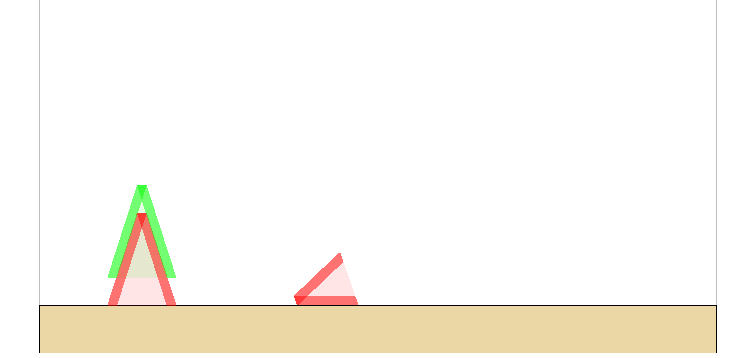
\includegraphics[width=0.2\textwidth]{rule1init_example}\\
\midrule
(2) Iota & $ N^{=}(\lambda\!x_1\!:~=\!(x_1, \mathrm{blue}, \mathrm{color}),1, \xx)$ (``there is exactly one blue cone'') &  \(\frac{\tau_{\mathrm{color}}}{810}\)  & 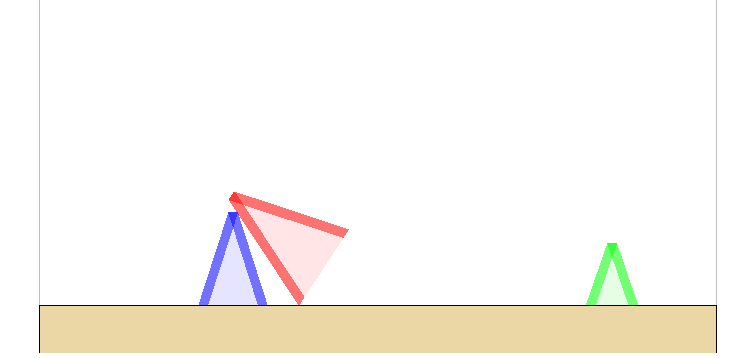
\includegraphics[width=0.2\textwidth]{rule4init_example}\\
  \midrule
(3) Upsilon & $\forall(\lambda\!x_1\!:~\neg(=\!(x_1, \mathrm{upright}, \mathrm{orientation})),X)$ (``no cone is upright'') &  \(\frac{\tau_{\mathrm{orientation}}}{270}\)  & 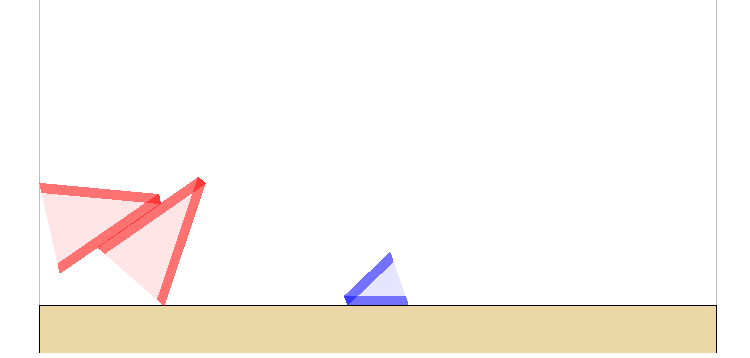
\includegraphics[width=0.2\textwidth]{rule3init_example}\\
 \midrule
(4) Kappa & $\exists(\lambda\!x_1\!:~\land\!(=\!(x_1,  small, \mathrm{size}), =\!(x_1, \mathrm{blue}, \mathrm{color}), X)$ (``there is a small blue cone'') & \(\frac{\tau_{\mathrm{size}}\times \tau_{\mathrm{color}}}{450}\) & 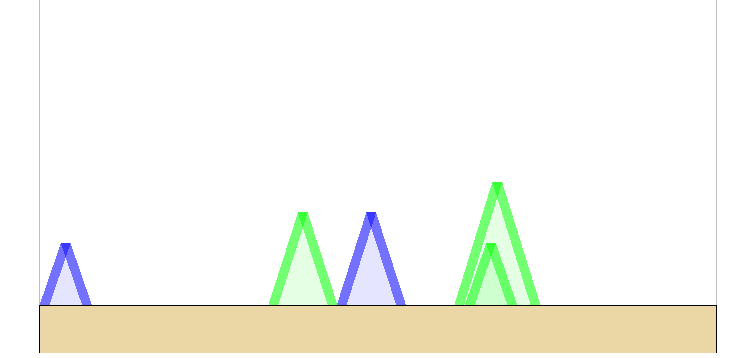
\includegraphics[width=0.2\textwidth]{rule5init_example}\\
  \midrule
(5) Omega & $\forall(\lambda\!x_1\!:~\lor\!(=\!(x_1,  small, \mathrm{size}), =\!(x_1, \mathrm{blue}, \mathrm{color}), X)$ (``all cones are small or blue'') & \(\frac{\tau_{\mathrm{size}}\times \tau_{\mathrm{color}}}{450}\) & 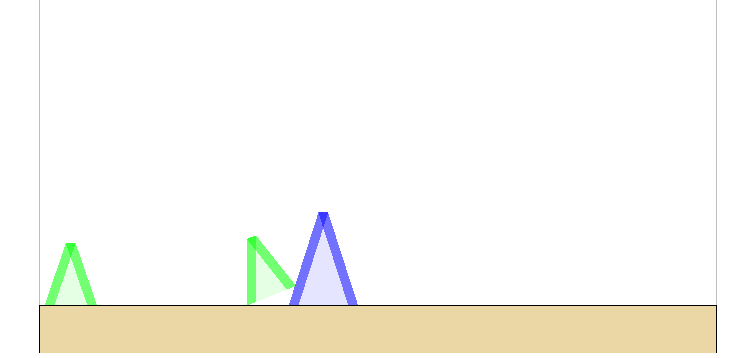
\includegraphics[width=0.2\textwidth]{rule6init_example}\\
\bottomrule
\end{tabular}
}
\label{table:table_2_rules}
}
\end{table}



\subsubsection{Procedure}
\paragraph{Initial Learning Phase} For each rule, participants first underwent a learning phase in which they observed one rule-following scene and subsequently created and tested seven scenes of their own (see Figures~\ref{fig:fig_1_zendo}-\ref{fig:fig_2_experiments}). Participants could add cones using the buttons shown at the bottom of Figure~\ref{fig:fig_1_zendo}a, remove cones via right-clicking on them or by holding left-click on them. They could rotate cones counterclockwise and clockwise using  ``Z'' and ``X'' respectively. Using the ``Test'' button, participants could then check whether the constructed scene followed the underlying rule or not and move on to their next test. Upon pressing ``Test'', scenes that followed the rule would be overlaid with a graphic of stars shooting upward and the message ``This arrangement DOES emit \{name of wave\} waves!'' was displayed while for non-rule-following scenes no stars would appear and the message ``This arrangement DOES NOT emit \{name of wave\} waves!'' appeared. Messages were displayed for one second. 


\paragraph{Initial Test Phase} 
After the (active) learning phase was a test phase. In this, participants were first asked to make generalization predictions about which of eight additional scenes were rule following (Figure~\ref{fig:fig_1_zendo}c). The test set for each rule contained four rule-following and four non-rule-following scenes selected from a large set of scenes created with a random scene generator and was the same for every participant. The true number of rule-following and not-rule-following scenes in this set was unknown to participants. 
Participants had to select at least one scene as rule following and fewer than all eight. While labelling test scenes, participants could see the summary of their initial test scenes (Figure~\ref{fig:fig_1_zendo}b). The positions of the rule-following and non-rule-following scenes were randomized between participants and trials. Participants then provided a free-text typed guess of the hidden rule (i.e., their initial hypothesis $\hi$ about the possible cause(s) of radiation). The response box required at least 15 characters. Underneath the textbox were bullet points asking participants to be as specific and unambiguous as possible and reminded them that the hidden rule could be related to any of the properties of cones and was unaffected by the previously created scenes.

\paragraph{Subsequent Learning and Final Test Phases}
Following the initial learning and generalization phase, participants were given the opportunity to perform seven additional experiments to discover the underlying rule. The procedure was identical to their initial active learning phase. Thereafter, participants were asked to revise their generalizations under consideration of the additional active learning data. Their initial selections were displayed during this revised generalization phase (Figure~\ref{fig:fig_2_experiments}). Finally, participants provided a second written response of their best guess of the hidden rule $\hr$. Participants were paid a performance bonus of 5 cent for each correctly selected test scene (max. bonus = 5 cent $\times$ 8 selections per trial $\times$ 5 trials = \$2.00). We did not provide performance feedback between trials (i.e., participants did not receive feedback about the accuracy of their generalizations or explicit rule guesses).


\subsubsection{Analysis Strategy}
\paragraph{Primary Analysis}
We will first report participants' generalization accuracy comparing it against that expected under rules sampled from the posterior.\footnote{For this we used the best fitting likelihood shape parameter $b$; see Model Comparison, for details.} Next, we assess how frequently participants and posterior-sampled hypotheses line up with the correct rule. Finally, we examine explicit changes to rule elements between initial ($\hi$) and revised ($\hr$) rule guesses to motivate our adaptation proposal.

\paragraph{Free Response Coding}
To analyze participants' explicit guesses about the rule in detail, we had two human coders convert participants' text responses into the first order logic and lambda abstraction format we use in our grammar wherever this was possible to do unambiguously. The human coders were trained on the grammar and blind to the relevant ground truths and instructed to preserve the syntactic structure and order used by the participant as far as possible. Coder 1 translated all free text responses into the grammar and Coder 2 independently checked and re-coded a random 15\% of the translated rules. Inter-rater agreements were 0.93 and 0.97 for Experiments 1 and 2, each higher than the 0.7 heuristic benchmark for adequacy \citep{krippendorff2018content}. Further details on our coding scheme and worked examples of the translation process are provided in Appendix~A-6.

\subsection{Results}

\begin{figure*}[!t]
    \begin{center}
    \begin{tikzpicture}
    \node[anchor=south west,inner sep=0] at (0,0) {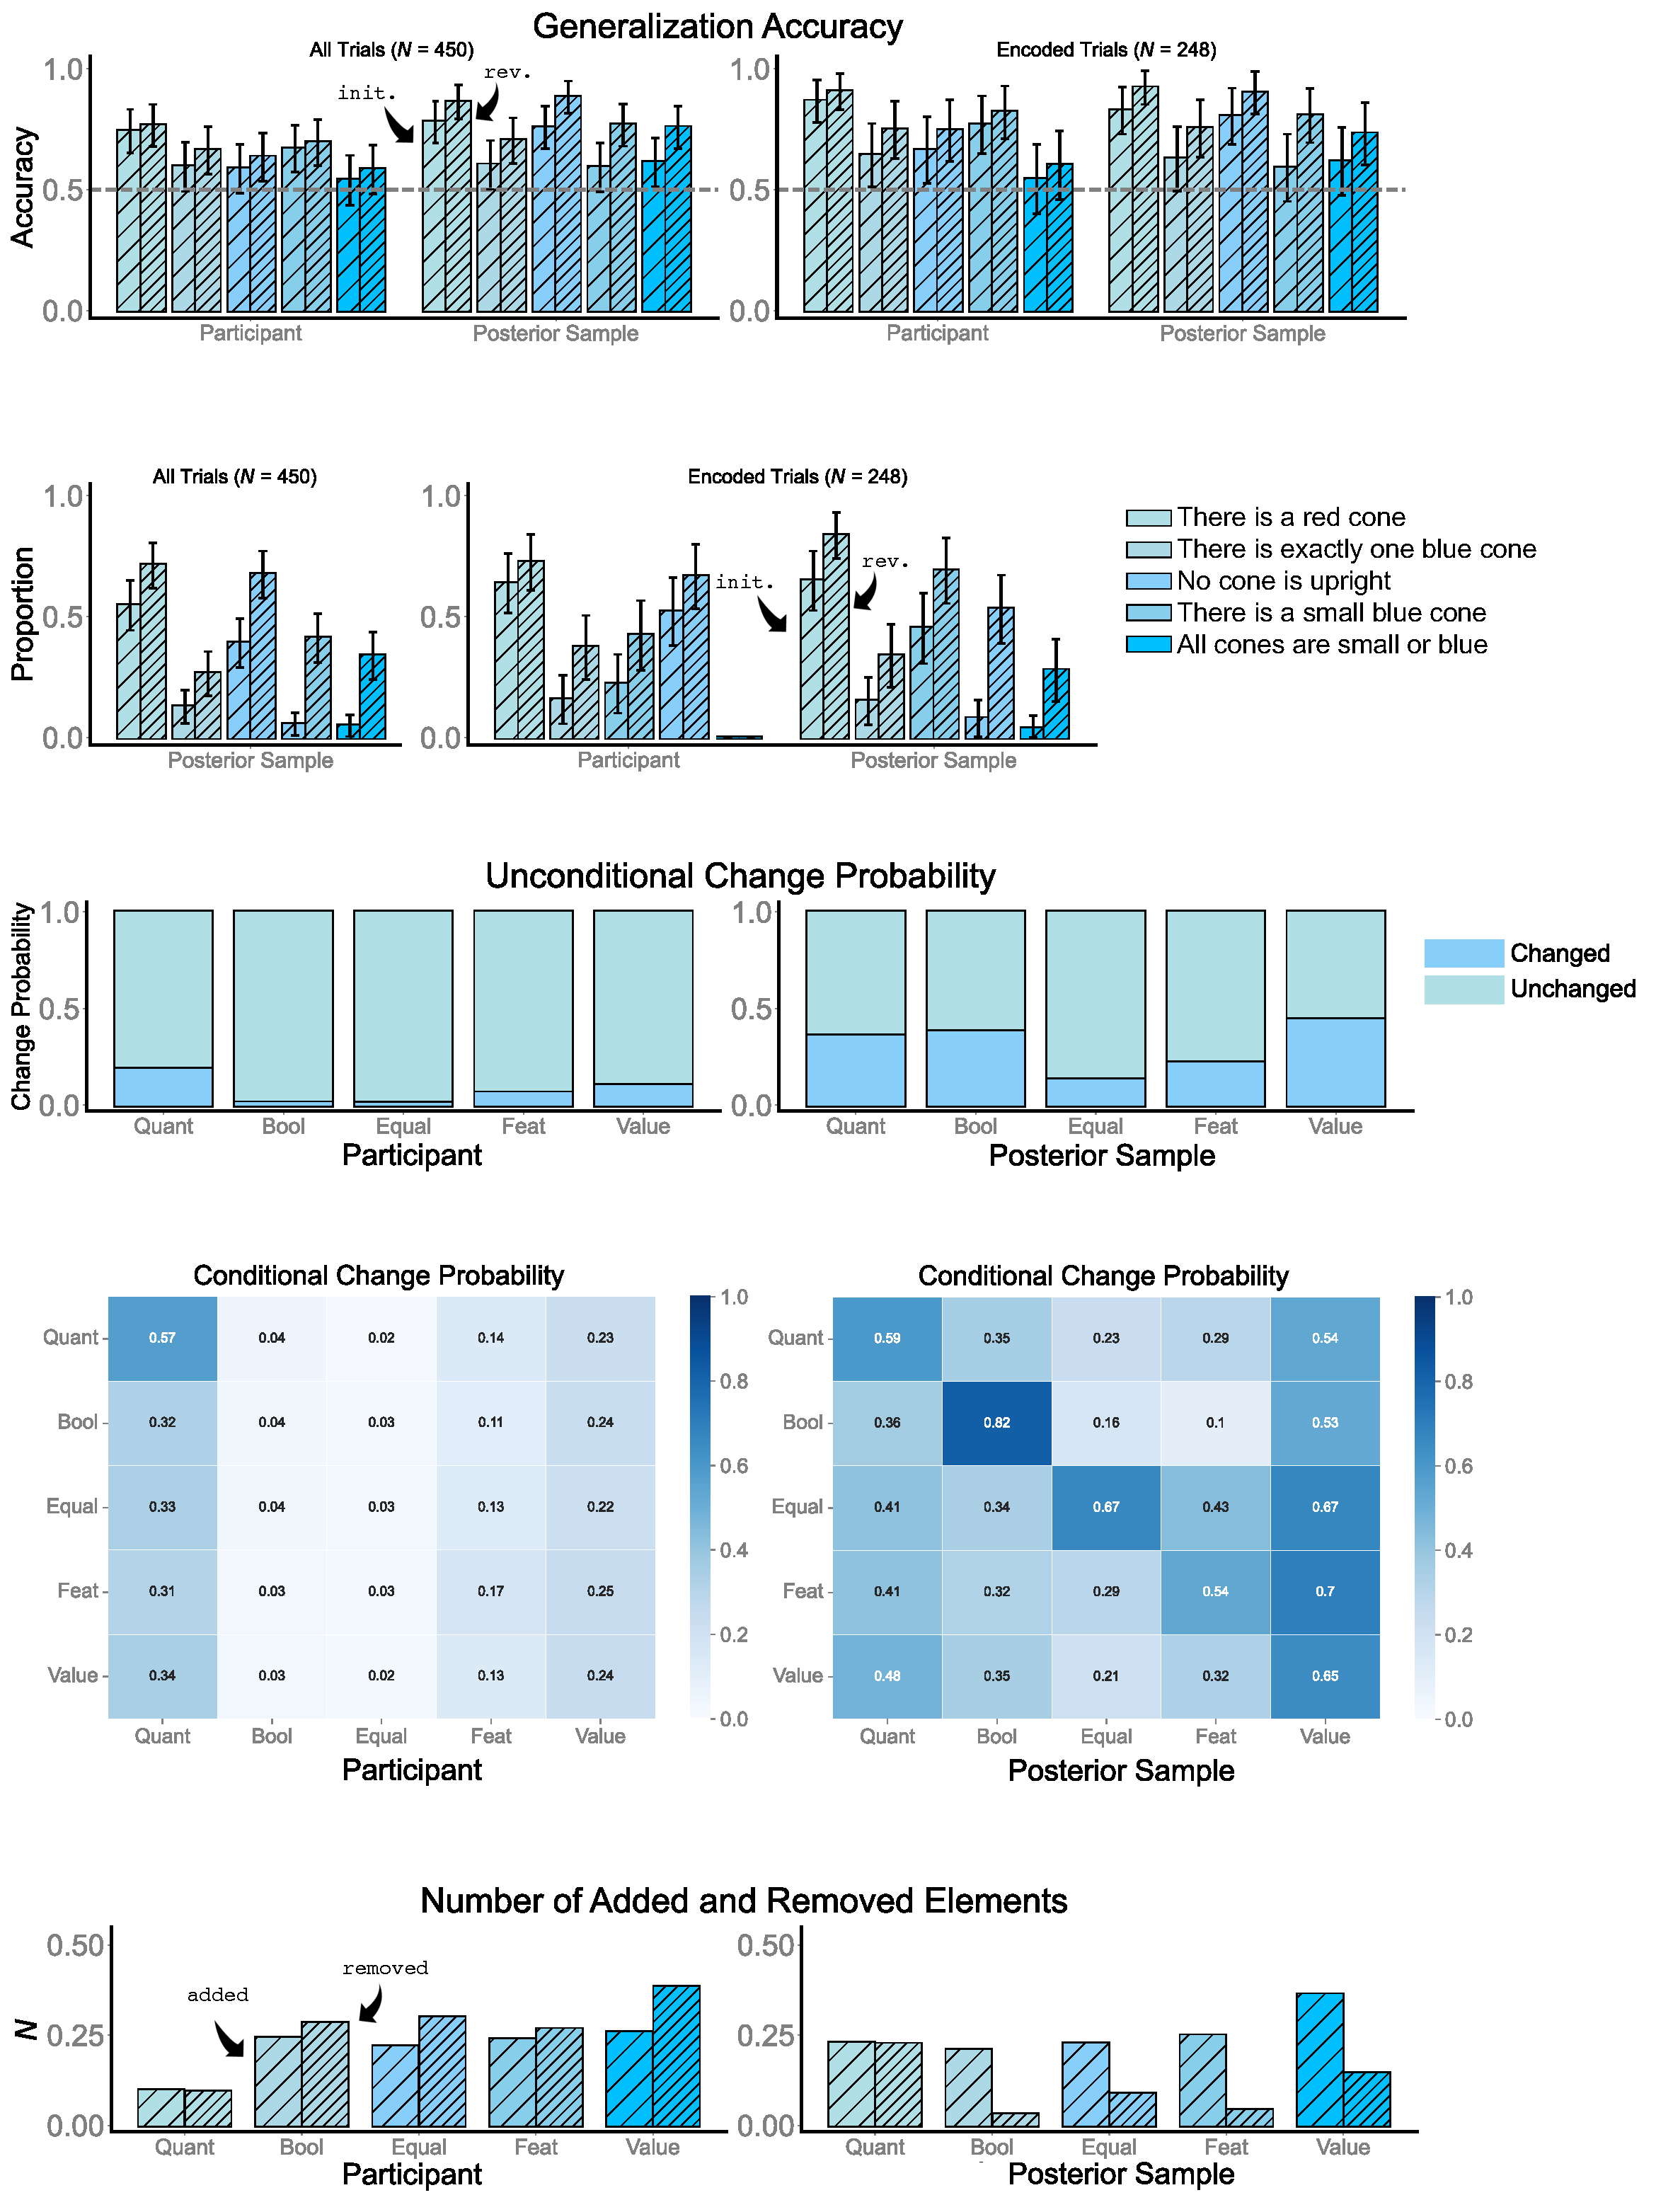
\includegraphics[width=.77\textwidth]{img/fig_5_exp_1_behavioural_res.pdf}};
    \draw (-0.25,15.6) node[below] {\textbf{$\mathsf{a)}$}};
    \draw (-0.25,12.6) node[below] {\textbf{$\mathsf{b)}$}};
    \draw (-0.25,9.6) node[below] {\textbf{$\mathsf{c)}$}};
    \draw (-0.25,6.85) node[below] {\textbf{$\mathsf{d)}$}};
    \draw (-0.25,2.3) node[below] {\textbf{$\mathsf{e)}$}};
    \end{tikzpicture}
    \end{center}
    \caption{Experiment 1. a) Generalization accuracy split by rule. b) Proportion of rule guesses semantically equivalent to ground truth (all trials and encoded trials for the posterior sample) and proportion of participants' encoded rule guesses semantically equivalent to ground truth split by rule. c) Unconditional change probability of each rule element (how often elements changed between $\hi$ and $\hr$ irrespective of changes to other elements). d) Conditional change probability of each rule element (how often elements changed between $\hi$ and $\hr$ conditional on changing a specific rule element). e) Average number of added and removed rule elements per trial. Error bars correspond to binomial CI.}
    \label{fig:fig_5_exp_1_behavioural_res}
\end{figure*}


\paragraph{Generalization Accuracy}
Participants correctly labelled 62.6$\pm$12.6\% of the generalization scenes after the initial learning phase, and this increased to 66.8$\pm$16.1\% after the second learning phase (Figure~\ref{fig:fig_5_exp_1_behavioural_res}a). Generalization accuracy thus improved significantly from phase one to phase two, as shown by a linear mixed-effects regression using revision as fixed predictor of accuracy and including random intercepts for both participants and rule types ($\beta$ =  0.042, $p$ $<$ 0.001). Generalization accuracy for simulated normative posterior guesses based on the data generated by participants showed a similar pattern going from 66.9$\pm$7.9\% in phase one to 79.5$\pm$11.3\% when based on all the learning evidence in phase two ($\beta$ = 0.126, $p$ $<$ 10$^{-10}$). The pattern of the results for the 248 trials with encodeable free responses was similar to that for the full dataset, with participants' generalization accuracy increasing from 70.5$\pm$14.0\% to 77.1$\pm$15.8\% ($\beta$ = 0.066, $p$ $<$ 0.001) and 69.7$\pm$9.7\% to 82.5$\pm$9.6\% ($\beta$  = 0.128, $p$ $<$ 10$^{-15}$) for posterior sampled hypotheses given the same evidence. 

\paragraph{Rule Guesses}
We next analyzed the frequency with which participants and posterior samples resulted in rule guesses semantically identical to the ground truth \footnote{We established semantic identity by checking that the guessed or sampled rule labelled 500 randomly sampled test scenes identically to the ground truth.}. Overall, participants guessed the rule correctly 32.3$\pm$24.0\% of the time after the initial learning phase and 45.2$\pm$29.2\% after the revised learning phase. This was commensurate with the probability of a normative posterior sample lining up exactly with the ground truth in 28.7$\pm$17.3\% after the initial learning phase and 54.5$\pm$20.7\% after revision. Figure~\ref{fig:fig_5_exp_1_behavioural_res}b breaks this down by rule, revealing that participants' guesses and posterior samples were similarly accurate for rules 1--3, while for rule 4 (``there is a small blue cone''), participants were more likely to guess correctly than posterior sampling. For rule 5  (``all cones are small or blue''), no participant 
guessed correctly with their initial ($\hi$) or revised $(\hr)$ guess, while posterior samples did occasionally land on the correct rule for the revised guess based on all data $P(H\mid\di,\dr)$. Table~\ref{table:table_3_rule_fitness} shows that participants' rules were more complex than the posterior samples (shown by the fact that they have a smaller average prior generation probability). The likelihood (fit) of participants' rule guesses was also lower than that for the posterior sampled rules. 


\begin{table}[!th]
\begin{center} 
\small
\caption{Mean ($\pm SD$) log prior generation probability and fit (loglikelihood) for participants' guesses and posterior rule samples using $b$ = 5.} 
\label{sample-table} 
% \begin{tabular}{c $C$ c $C$ c $C$ c $C$ c}
\resizebox{\columnwidth}{!}{
\begin{tabular}{c c c c c c} 
Exp. & Learner & $\log P(h_{init.}) $ & $\log P(h_{rev.})$ & $\log P(D_{init.}\mid h_{init.},b) $ & $\log P(D_{init.,rev.}\mid h_{rev.},b)$\\
\toprule
 \multirow{2}{*}{Exp. 1} & Participants & $-3.61 \pm0.60$ & $-3.56\pm0.62$ & $-4.64\pm5.97$ & $-10.22 \pm 10.71$ \\
& Posterior Sample & $-2.71\pm0.12$ & $-2.90 \pm0.20$ &  $-1.53\pm0.87$ & $-2.97\pm1.76$ \\
\midrule
\multirow{2}{*}{Exp. 2} & Participants & $-3.58\pm0.53$ & $-3.58\pm0.56$ & $-5.51\pm5.28$ & $-13.94\pm10.37$\\
& Posterior Sample & $-2.71\pm0.11$ & $-2.93\pm0.19$ &  $-1.49\pm1.01$ &  $-3.19\pm1.86$ \\
\bottomrule
\label{table:table_3_rule_fitness}
\end{tabular} 
}
\end{center} 
\vspace{-.75cm}
{\notesize Prior generation probabilities are based on the polynomial adjustment (see Appendix~A-1 Equation~\ref{equ:equ_a1_2_kappa}).}
\end{table} 

\subsubsection{Explicit Rule Changes}
To assess whether there is qualitative support for our incremental hypothesis adaptation proposal, we next investigated whether participants' exhibit patterns of anchoring between their initial and revised guesses. Following previous work on anchoring effects \citep{dasgupta2017hypotheses, bramley2017formalizing, lieder2018anchoring}, we hypothesized that participants would tend to retain elements of their initial rules while adapting others, leading to non-normatively high levels of similarity between initial and revised guesses. Of course there are normative reasons to expect similarity between initial and revised guesses --- often the additional data will not overturn the earlier guess --- as well as cases where we expect a complete change --- such as when the new evidence leads to a completely new hypothesis being favored. Thus, as well as low overall change to hypotheses, we also expect anchoring to manifest in small proportions of conditional changes. That is, if learners tend to tweak just a few elements in their initial hypothesis to arrive at their revised hypothesis, we expect that conditioning on there being a change in one element of a participant's hypothesis, there should be a relatively low probability of other elements also changing compared to a change pattern between two independent posterior samples. 

To explore the relationship between initial and revised guesses, we visualize the absolute proportion of change in each rule element type (Figure~\ref{fig:fig_5_exp_1_behavioural_res}c) as well the degree of change conditional on other changes (Figure~\ref{fig:fig_5_exp_1_behavioural_res}d) comparing against independent posterior sampling in each case (for details on how we calculated conditional changes, see Appendix~A-7). This reveals that participants revise their hypotheses much more locally, making few changes overall and having much lower conditional change probabilities -- i.e., less tendency to changing multiple elements in combination. We note that while the absolute amount of change between an initial and revised posterior sample depends on the strength of the prior and likelihood function, we would still expect participants' heatmap pattern of ``internal'' conditional changes to resemble that of normative sampling if their revised guess is independent of their initial guess. However, we see a markedly different pattern in Fig.~\ref{fig:fig_5_exp_1_behavioural_res}d with very low conditional change probabilities across the board for participants. Finally, we separately consider the number of added and removed rule elements. Figure~\ref{fig:fig_5_exp_1_behavioural_res}e shows that, on average, participants removed slightly more rule elements than they added going into their final judgment, while independent posterior samples have the opposite pattern, tending to increase in complexity in phase two when more evidence is available, excepting the number of quantifiers (and hence bound variables). The general increase in complexity makes sense since more evidence licences more complex theories (with patterns in the data playing a relatively greater role and the prior preference for simpler rules having relatively less impact). The smaller number of quantifiers might reflect that revised normative samples also better lined up with the true conjunctive and disjunctive rules (``there is a small blue cone'', ``all cones are small or blue'') which, in this experiment, only ever required a single quantifier (Figure~\ref{fig:fig_5_exp_1_behavioural_res}b).

\subsection{Discussion of Experiment 1}
In Experiment 1, we saw that participants improved the quality of their guesses after gathering additional active learning data. This was true in terms of the accuracy of their generalizations, but also in terms of how often their explicit rule guesses matched the ground truth. Participants' performance in terms of generalization and correct guesses was broadly commensurate with that of posterior sampling. However, a closer analysis of explicit rule changes suggests that participants' pairs of guesses were substantially anchored to one another. We take this as qualitative support for our idea that participants often revise their hypothesis through limited local adaptation starting from their initial hypothesis in the light of the additional learning data. 

\section{Experiment 2 - Dyadic Yoked Learning}
\subsection{Methods}
\subsubsection{Participants}
Forty-two participants (making up 21 dyads; age 35.30$\pm$10.51 years [M$\pm$SD]) were recruited from Amazon's Mechanical Turk (hit approval rate $\geq$ 95\%) and paid as in Experiment 1. To enable real-time interaction between paired participants, we used {\tt Socket.IO}. Similar to Experiment 1, not all of the 210 free responses could be unambiguously translated into our grammar.  %127 of the 210 free responses could be unambiguously translated into our grammar. 
Trials with ambiguous ($N=45$) or nonsensical ($N=38$) rule guesses were only included in the primary analysis and model comparisons are based on the 127 encoded trials. 

\subsubsection{Procedure}
The initial active learning and generalization phases were identical to Experiment 1. However, after this, participants were shown the active learning data produced by their learning partner, and vice versa. As with Experiment 1, participants then had the opportunity to provide updated generalizations and an updated guess about the true rule. Both the participants' own learning data and initial selections and the experiments performed by their partner were displayed during revision (see Figure~\ref{fig:fig_2_experiments}). Our analyses of Experiment 2 will follow the same structure as Experiment 1. 


\subsection{Results}

\begin{figure*}[!t]
    \begin{center}
    \begin{tikzpicture}
    \node[anchor=south west,inner sep=0] at (0,0) {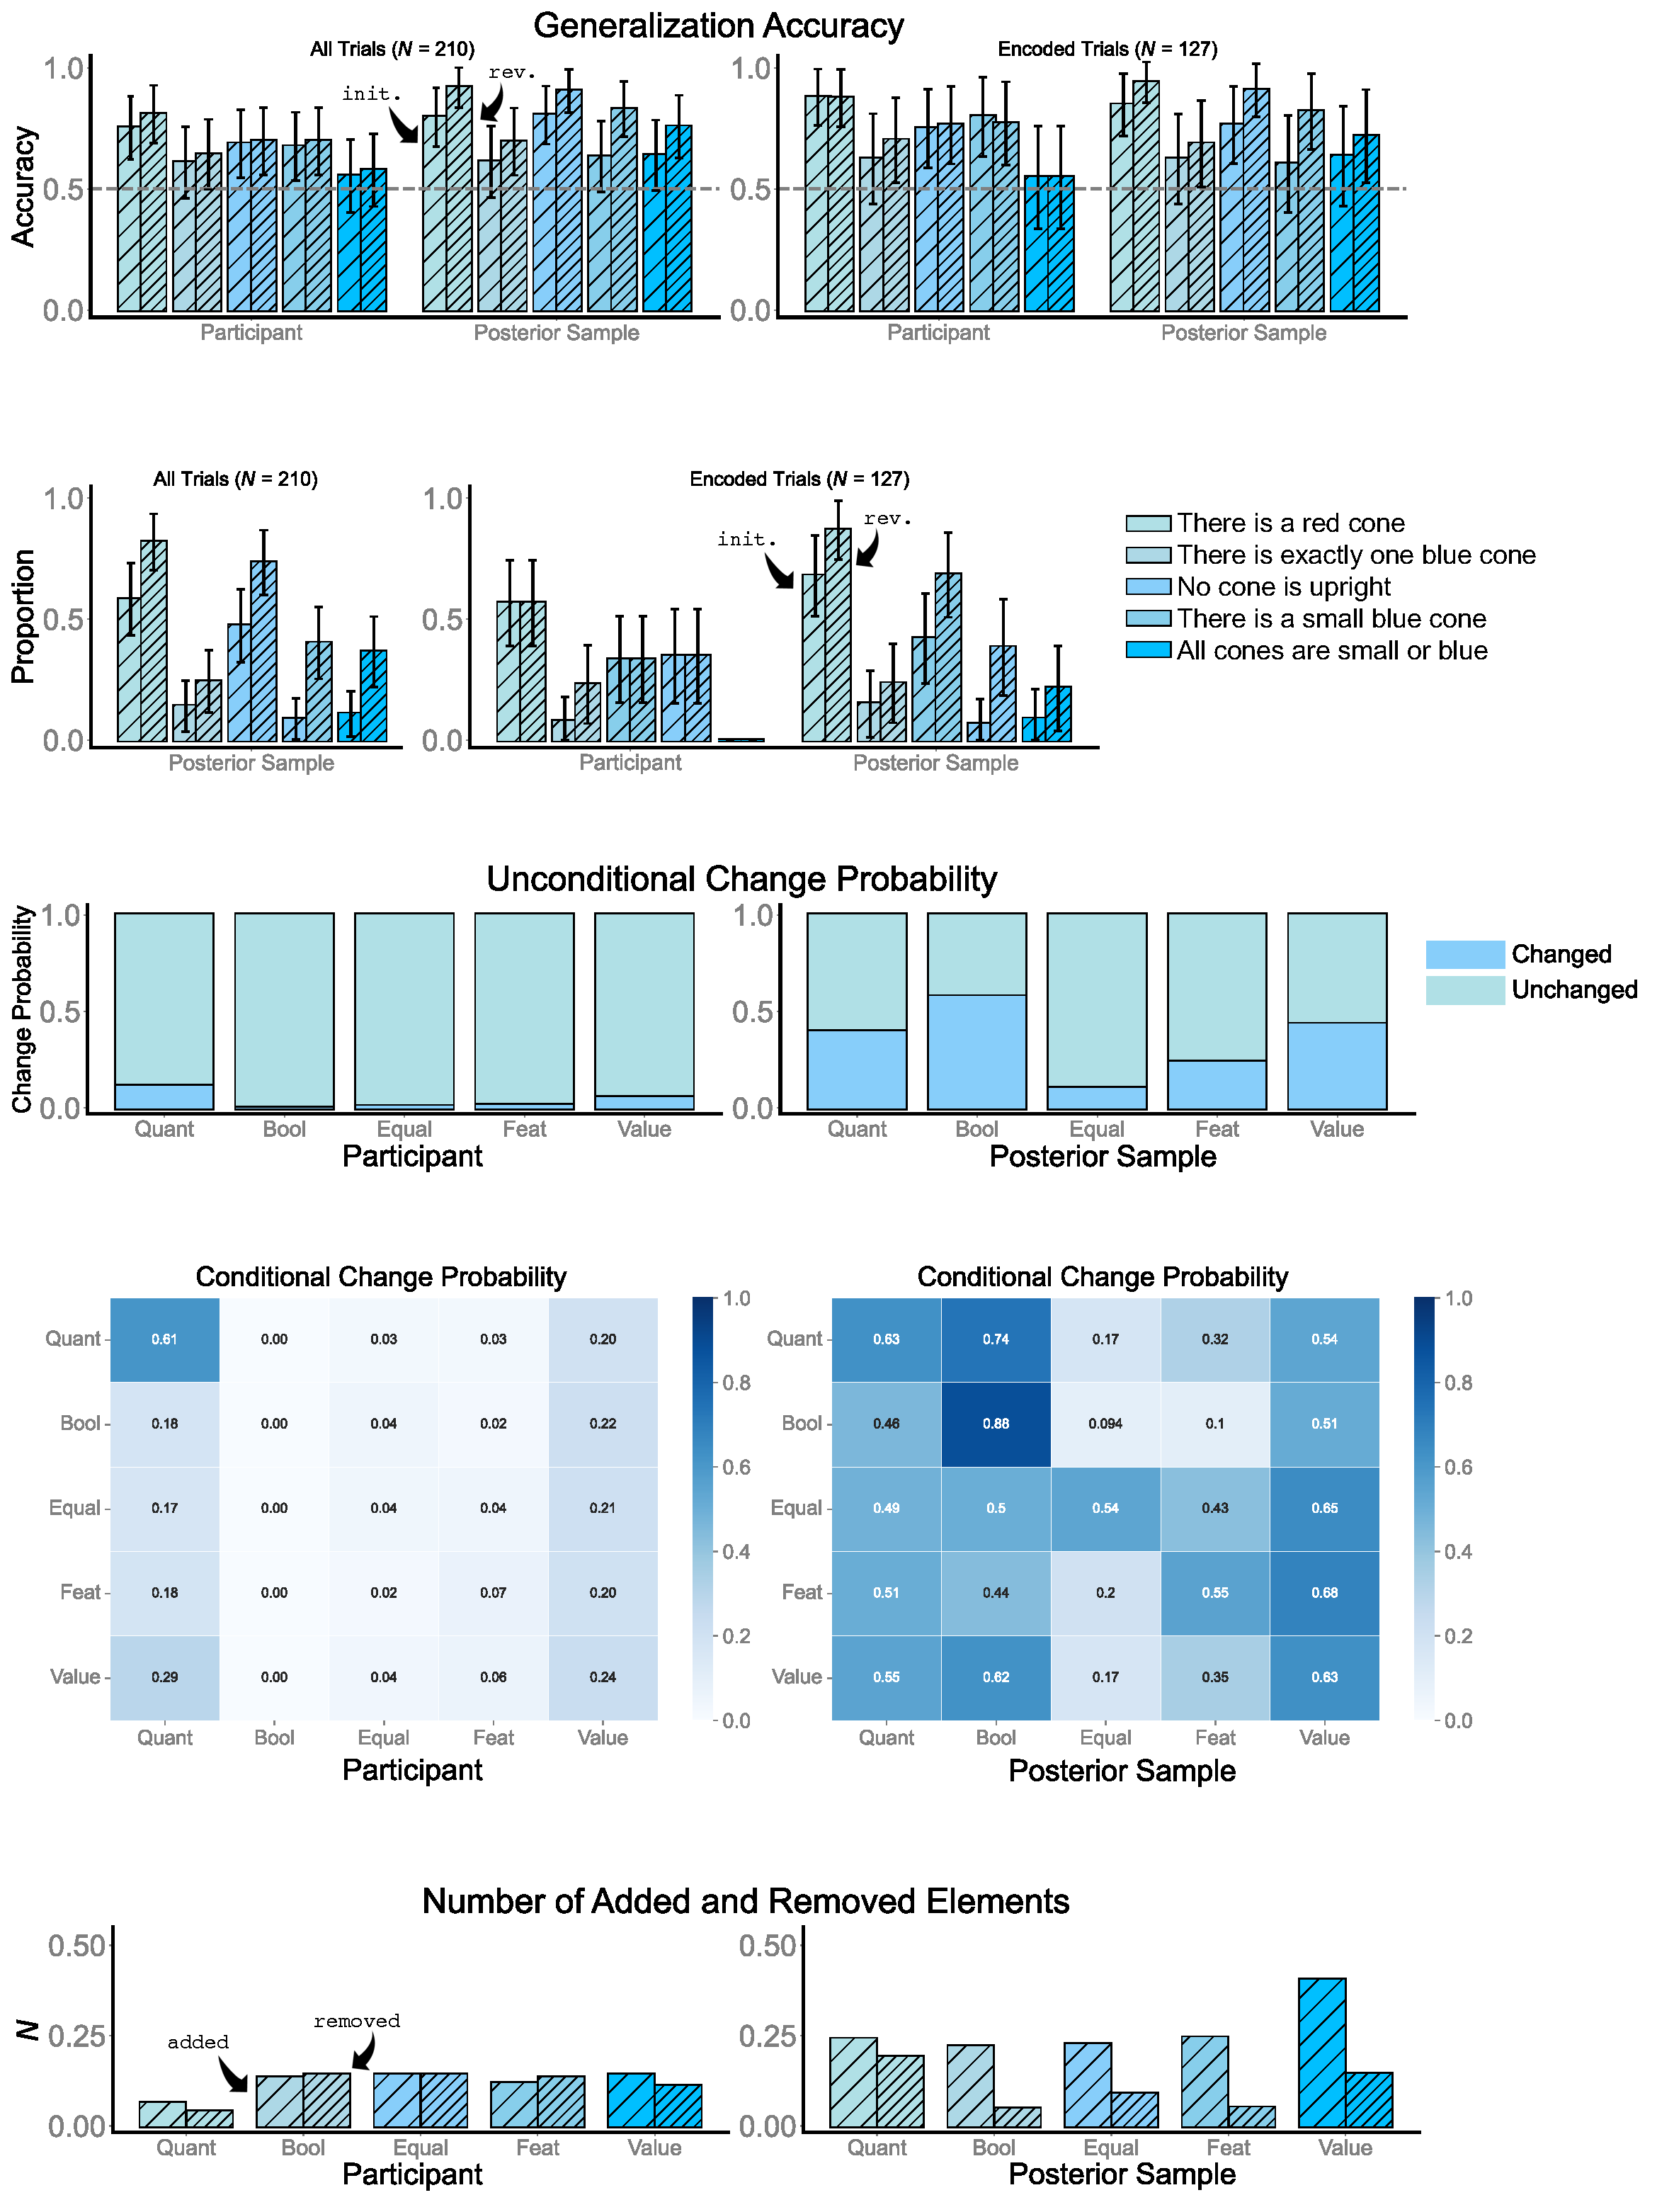
\includegraphics[width=.77\textwidth]{img/fig_6_exp_2_behavioural_res.pdf}};
    \draw (-0.25,15.6) node[below] {\textbf{$\mathsf{a)}$}};
    \draw (-0.25,12.6) node[below] {\textbf{$\mathsf{b)}$}};
    \draw (-0.25,9.6) node[below] {\textbf{$\mathsf{c)}$}};
    \draw (-0.25,6.85) node[below] {\textbf{$\mathsf{d)}$}};
    \draw (-0.25,2.3) node[below] {\textbf{$\mathsf{e)}$}};
    \end{tikzpicture}
    \end{center}
   \caption{Experiment 2. a) Generalization accuracy split by rule. b) Proportion of rule guesses semantically equivalent to ground truth (all trials and encoded trials for the posterior sample) and proportion of participants' encoded rule guesses semantically equivalent to ground truth split by rule. c) Unconditional change probability of each rule element (how often elements changed between $\hi$ and $\hr$ irrespective of changes to other elements). d) Conditional change probability of each rule element (how often elements changed between $\hi$ and $\hr$ conditional on changing a specific rule element). e) Average number of added and removed rule elements per trial. Error bars correspond to binomial CI.}
    \label{fig:fig_6_exp_2_behavioural_res}
\end{figure*}



\paragraph{Generalization Accuracy}
Participants correctly labelled 65.5$\pm$11.8\% of the generalization scenes after phase one and this increased to 68.5$\pm$11.9\% after seeing their partner's data (Figure~\ref{fig:fig_6_exp_2_behavioural_res}a). Unlike Experiment 1, this increase was not statistically significant ($\beta$ = 0.029, $p$ = 0.154). However, the predictive accuracy of normative posterior samples increased from 69.8$\pm$7.6\% to 82.2$\pm$6.6\% ($\beta$ = 0.124, $p$ $<$ 10$^{-10}$) indicating that the additional data was informative in principle. Similarly, for the 127 trials in which participants made two unambiguous rule guesses, initial generalization accuracy 73.0$\pm$11.7\% did not differ from
final accuracy (74.3$\pm$11.9\%; $\beta$ = 0.013, $p$ = 0.561), while the posterior sample improved from 70.5$\pm$9.3\% to 82.3$\pm$8.6\% ($\beta$ = 0.118, $p$ $<$ 10$^{-09}$).


\paragraph{Rule Guesses \& Anchoring}
Replicating the pattern from Experiment 1, we found that participants showed commensurate overall accuracy as posterior samples. In Experiment 2, participants' rule guesses aligned with the ground truth in 28.3$\pm$18.1\% of the time after the initial learning phase and  31.5$\pm$20.0\% after revision, while the posterior sample had a match of 30$\pm$19.7\% after the initial learning phase and 50$\pm$20.1\% after revision (Figure~\ref{fig:fig_6_exp_2_behavioural_res}b). Participants again outperformed posterior sampling for rule 4 (``there is a small blue cone'') but this time only with their initial guess. They again failed to guess rule 5 correctly for either initial or revised responses. Unlike Experiment 1, participants showed little improvement from initial to revised guesses, with the proportion guessing correctly improving only for rule 2 (``there is exactly one blue cone''). The pattern of prior generation probabilities and rule fits matched the findings from Experiment 1 with participants again producing somewhat more complex and less well fitting guesses than would be expected under normative posterior sampling (Table~\ref{table:table_3_rule_fitness}).

For participants, both the unconditional changes (Figure~\ref{fig:fig_6_exp_2_behavioural_res}c) and conditional changes (Figure~\ref{fig:fig_6_exp_2_behavioural_res}d) to rule elements between their initial and revised guesses were lower than in Experiment 1 and with a different pattern to the independent posterior sampling pattern. This is again consistent with our hypothesis that revisions are made through limited local edits. Compared to Experiment 1, participants were also less likely to add or remove rule elements. To the extent that they did, they tended to remove more Booleans, equalities and features than add them while the pattern for the normative learner was almost identical to Experiment 1, showing more additions than removals overall (Figure~\ref{fig:fig_6_exp_2_behavioural_res}e).
 
 
\subsection{Positive Testing and Hypothesis Adaptation}

We next sought to better understand why participants' accuracy increased in Experiment 1 while there was no significant difference as a function of revision in Experiment 2. We hypothesized based on past work \citep{wason1960failure, klayman1987confirmation} that participants frequently generate tests that are likely to be rule following under their current hypothesis. Thus, we compared the proportion of such positive tests (i.e., test scenes following participants' initial explicit rule guess $\hi$) during the revised learning phase across experiments using a binomial mixed-effects regression with Experiment (1 vs 2) as fixed effect predicting test scene (scene follows $\hi$ = 1, scene does not follow $\hi$ = 0) including random intercepts for both participants and rules. This revealed a significant decrease in the proportion of positive tests from 68.5$\pm$15.4\% in Experiment 1 to 53.5$\pm$23.7\% in Experiment 2 ($\beta$ = -0.784, $p$ $<$ 0.001). This confirms that actively gathered data in the phase two of Experiment 1 indeed bears hallmarks of confirmatory or positive testing, while by design this does not hold in Experiment 2. 

\subsection{Discussion of Experiment 2}
In Experiment 2, we found that seeing additional active learning data coming from a partner did not allow participants to improve the quality of their generalizations or their guesses. Though the average pattern of results was similar to Experiment 1 (i.e., revised generalization accuracy was higher than initial generalization accuracy), looking at accuracy per rule for encoded trials showed that participants' revised generalization accuracy for the rule ``there is a red cone'' and the rule ``there is a small blue cone'' was slightly lower than their initial generalization accuracy for these rules. Our analysis of rule guesses provided further insight into the differences between experiments. Participants' guesses only improved for 1 of the 5 rules, suggesting that seeing active learning data collected by someone else did not benefit them in the same way as additional active learning data had in Experiment 1. Our analysis of explicit rule changes suggested even greater degrees of anchoring than that found in Experiment 1 with participants making very few changes to their hypotheses on average when seeing their partners' data despite this data being valuable from a normative perspective.


\section{Model Comparison}

In order to quantitatively examine our conjecture that participants locally adapted their initial hypotheses to form their revised hypotheses, we now compare a range of computational and process level models to participants' guesses and generalizations. We compared seven models in total, fitting one or two parameters in each case using a coarse grid search, and using the Bayesian Information Criterion \citep[BIC,][]{schwarz1978estimating} as our metric of model quality. The models we considered were: (1) $\hi$ as a baseline, (2) Posterior Sampling (PS), (3) Maximum a posteriori (MAP), (4) Win--Stay, Lose--Sample (WSLS), local adaptation by (5) Tree Regrowth (TR) and (6) Tree Surgery (TS), and (7) a modified form of RULEX that we refer to as RULEX* in our results.

We hypothesize that a local adaptation model (TR or TS) will better capture participants' revised judgments than the models that treat each guess as independent (Posterior Sampling or MAP). Furthermore, we hypothesize that the kinds of edits participants make may be better characterized by a local ``Tree Surgery'' (TS) than the more mobile ``Tree Regrowth'' (TR) algorithm. We also hypothesized that participants do not always stick with their initial hypothesis ($\hi$), will diverge from Win--Stay, Lose--Sample's all-or-none dependence pattern, and also from a heuristic RULEX*-style search.

\paragraph{Parameters}
For each model, we fit a likelihood parameter with a coarse grid search $b\in \{1, 3, 5, 7, 9\}$. This grid corresponds to a likelihood with which a rule mislabels a given scene that ranges from a highly stochastic $e^{-1}=0.37$ to a practically deterministic $e^{-9} = 0.0001$; see Equation~\ref{equ:equ_3_likelihood}). For TR, TS and RULEX* we assume each search is performed for a finite number of steps $k \sim \mathrm{Poisson}(\lambda)+1$ (see Equation~\ref{equ:equ_7_poisson}), where we examine $\lambda \in \{0.5, 0.75, 1, 3, 10\}$.

\paragraph{Evaluating the models}
We first considered two computational level accounts: Posterior Sampling, and selection of the MAP hypothesis. Since the posterior probability of $\hr$ is independent of $\hi$ conditional on the data, we can estimate the likelihood of drawing $\hr$ as an independent posterior sample by simply counting how frequently a posterior sample based on all learning data faced by a participant exactly matches the participant's revised guess $\hr$. If $\hr$ did not appear at all in a sample of 10,000 posterior hypotheses, we fall back on an $\epsilon$ likelihood of $\frac{1}{10,000}$.\footnote{We examine this choice in Appendix~A-8.} For the MAP, we identify the most likely hypothesis (or joint most likely hypotheses) in a sample of 10,000 and assign a likelihood of 1 if $\hr$ was equal to the MAP hypothesis or $\epsilon$ for trials in which the MAP hypothesis was not equal to $\hr$. Both these models have one free parameter $b$ controlling the impact of mislabeling on the likelihood of rules (see Equation~\ref{equ:equ_3_likelihood}).

As a baseline, we also considered whether participants might be described as simply keeping $\hi$ (resulting in a likelihood of 1 if $\hr=\hi$ or of $\epsilon$ otherwise). 
We then also considered Win--Stay, Lose--Sample (WSLS). For this, we take a mixture between predicting a match with a participant's initial guess (likelihood of 1 if $\hr=\hi$ and $\epsilon$ otherwise) with mixture weight $P(\dr\mid\hi, b)$ and a predicted selection of an independent posterior sample as above, with mixture weight $1-P(\dr\mid\hi, b)$. This model also had one free parameter $b$ affecting both the chance of re-sampling and the shape of the posterior being resampled from.

For the TR and TS local adaptation models, we estimated the likelihood of a participant's $\hr$ by starting with a participant's initial rule guesses $\hi$ and running many MCMC adaptation chains. We used inverse binomial sampling \citep{van2020unbiased} to estimate the reciprocal of the likelihood that a given chain with proposal distribution (TR or TS) and mean search length $\lambda+1$ would terminate in that participant's $\hr$. Essentially, this involved tracking how many chain attempts it took on average before a chain ended on a participant's judgment. 
For each combination of $b$ and $\lambda$, we simulated each adaptation algorithm repeatedly until it either produced a participant's final rule guess exactly or reached a time-out threshold (which we set to 100 to maintain computational tractability). We repeated this process 100 times for each participant's guess and averaged the resulting $\frac{1}{N_{\mathrm{attempts}}}$ values as the likelihood of generating $\hr$, taking timeouts as zeros and falling back on a likelihood of $\epsilon$ if $\hr$ was never generated. We nested the TR and TS proposals within WSLS. That is, we assumed participants updated their hypothesis with probability $1-P(\dr\mid\hi, b)$ or left it as it was initially with probability $P(\dr\mid\hi, b)$.

Finally, we based our implementation of RULEX on \cite{navarro2005analyzing}. Our RULEX* has several search phases: 1. Exact search (searching for a single feature rule that perfectly classifies all data points), 2. imperfect simple search (searching for a single feature rule that classifies most data points correctly, but now allowing for some exception(s)), and 3. conjunct-disjunct search (searching for a rule including either one conjunction or one disjunction that classifies most data points correctly, but allowing for some exception(s)). Whether imperfect simple or conjunct-disjunct search is performed after exact search is assumed to be random. In our task, we take simple rules to be any that refer to exactly one feature of the environment and contain no conjunctions or disjunctions. For example, ``there is a red cone'' or ``there is exactly one blue cone'' are simple in this sense. We take conjunctive rules to be those that include exactly one conjunction, such as ``there is a small blue cone'' or ``there is a red and exactly one blue''. Since our set of test rules also included a disjunctive rule (``all cones are small or blue'', see ground truth 5 in Table~\ref{table:table_2_rules}), we allow our RULEX* implementation to also generate disjunctive rules directly during the conjunct-disjunct search phase rather than requiring it to generate a conjunction of negations (e.g., ``all cones are not not small and not blue'').

Since RULEX has no mechanism for sampling data-consistent rules directly, we conceived of search as generating hypotheses uniformly without replacement from the prior restricted to the complexity class and evaluating these against the evidence. For each stage of search, if one or more of the considered hypotheses meet the termination condition, this is selected (uniformly if there are several front runners) as the rule chosen by the algorithm (see Appendix~A-5, for further details). There are $528$ simple rules that can be generated from our grammar, and these contain our ground truths 1--3. There are at least $557,568$\footnote{$557,568$ can be seen as a lower bound estimate of a hypothesis space consisting of $528^2$ conjunctive rules and $528^2$ disjunctive rules. Since we allow for arbitrary negations and quantifications such as ``all cones are not not small and not blue'' the actual hypothesis space is larger than the lower bound.} possible conjunctive and disjunctive rules containing our ground truth 4 and ground truth 5. We allowed RULEX* a variable search capacity $k = \lambda +1 $ as with TR- and TS-Learners, again evaluating this at $\lambda \in \{0.5, 0.75, 1, 3, 10\}$. Note that if we allowed a large search capacity, such as $\lambda = 1000$, RULEX* would always find simple rules 1--3 provided they are unique among simple rules consistent with the evidence, but would rarely find conjunctive or disjunctive rules due to the much larger search space. To increase its competitiveness, we further assumed RULEX* started with participants' initial rule guesses $\hi$. That is, RULEX* included $\hi$ in its initial search phase (regardless of $\hi$'s complexity) and terminated with $\hi$ deterministically if $\hi$ accounted for all the evidence. If $\hi$ failed during exact search, RULEX* discarded $\hi$ and proceeded with its other search phases. We simulated 10,000 such search attempts for each trial of the experiment and counted how many terminated in $\hr$ with $\frac{N}{10,000}$ resulting as our estimate of the likelihood of RULEX* and falling back to an $\epsilon=\frac{1}{10,000}$ likelihood if no search attempt terminated in $\hr$.



\subsection{Modeling Results and Discussion}

\begin{table*}[!ht]
\begin{center} 
\caption{Best fitting model performances for participants' revised rule guesses ($\hr$).} 
\vskip 0.10in

\begin{tabular}{l r c c c c} 
\small
Experiment & Model & Mean $BIC_{\hr}$ & $N_{\text{Best}_{\hr}}$ & $b$ & $\lambda$ \\ 

\toprule
% exp 1
\multirow{7}{*}{Exp. 1} & $\hi$ & 8.988 & 22.17 & - & -\\
& $\text{Posterior Sample (PS)}$ & 9.817 & 6.00 & 5.0 & -\\
& $\text{Maximum a posteriori (MAP)}$ & 11.164 & 4.17 & 7.0 & -\\
& $\text{Win--stay, lose--sample (WSLS)}$ & 7.158 & 7.17 & 1.0 & -\\
& $\text{WSLS with Tree Regrowth (TR)}$ & 6.368 & 12.17 & 3.0 & 10.0\\
& $\text{\textbf{WSLS with Tree Surgery (TS)}}$ & \textbf{5.917} & \textbf{15.17} & \textbf{5.0} & \textbf{10.0}\\
& $\text{RULEX}^*$ & 9.202 & 2.17 & - & 10.0\\
\midrule
% exp 2
\multirow{7}{*}{Exp. 2} & $\hi$ & 5.657 & 16.37 & - & -\\
& $\text{Posterior sample (PS)}$ & 11.403 & 2.00 & 5.0 & -\\
& $\text{Maximum a posteriori (MAP)}$ & 12.367 & 1.17 & 7.0 & -\\
& $\text{Win--stay, lose--sample (WSLS)}$ & 6.573 & 0.37 & 1.0 & -\\
& $\text{WSLS with Tree Regrowth (TR)}$ & 4.473 & 3.37 & 1.0 & 1.0\\
& $\text{\textbf{WSLS with Tree Surgery (TS)}}$ & \textbf{4.065} & \textbf{10.37} & \textbf{1.0} & \textbf{1.0}\\
& $\text{RULEX}^*$ & 9.220 & 2.37 & - & 3.0\\
\bottomrule
\label{table:table_4_h_rev}
\end{tabular}
\end{center} 
\end{table*}

\begin{figure*}[!t]
    \begin{center}
    \begin{tikzpicture}
    \node[anchor=south west,inner sep=0] at (0,0) {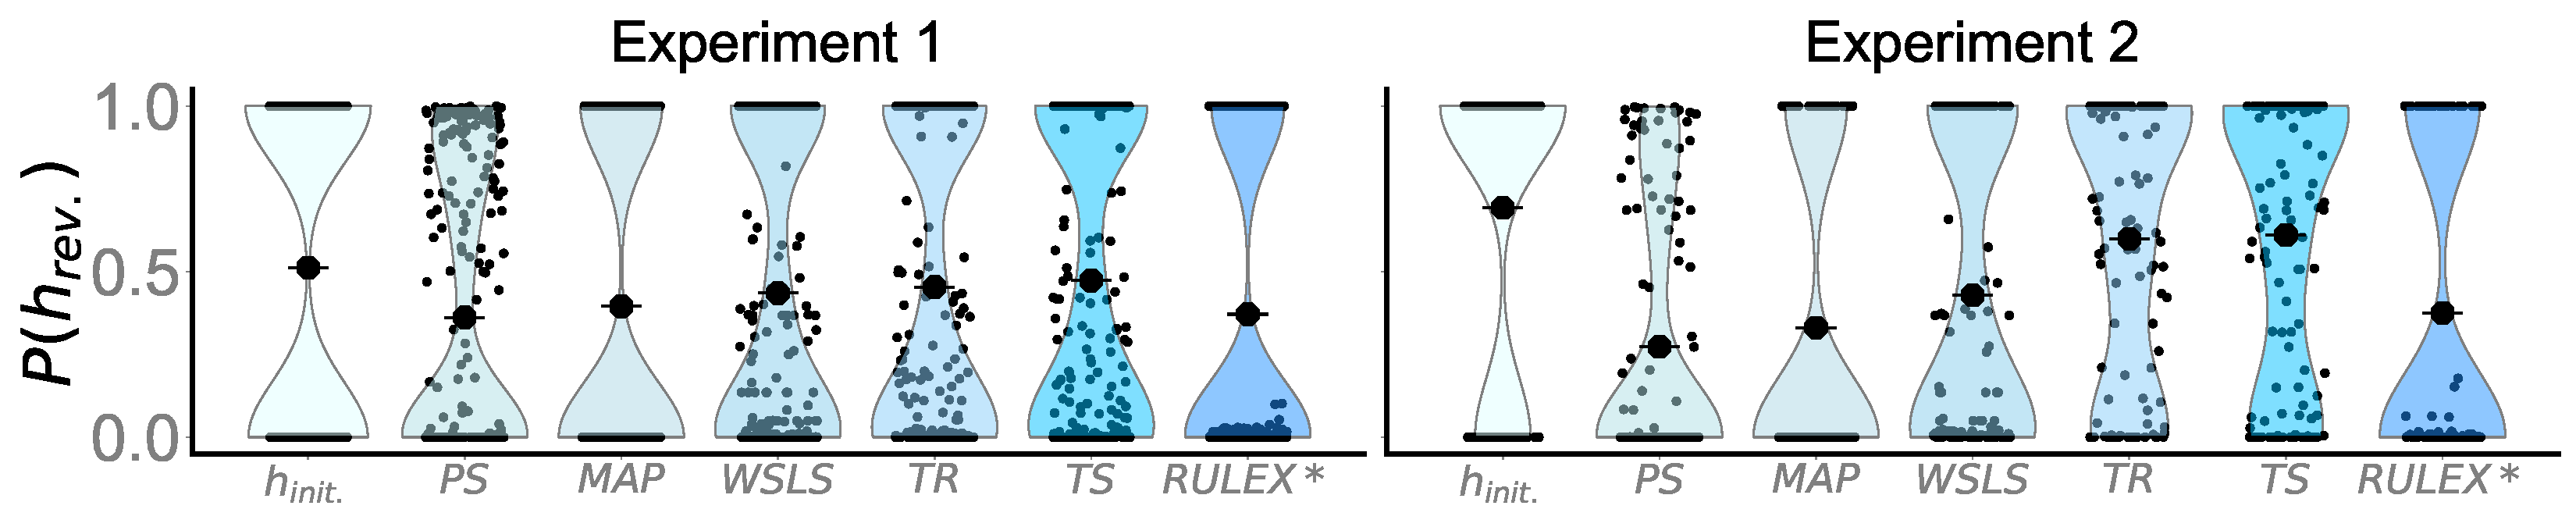
\includegraphics[width=.99\textwidth]{img/fig_7_mean_prob.pdf}};
    \end{tikzpicture}
    \end{center}
    \caption{Probability of participants' revised rule guess $\hr$ for each competing model using best fitting parameters (see Table~\ref{table:table_4_h_rev}). Points are individual trials and violin plots were generated using {\tt violinplot} \citep{hunter2007matplotlib} with a default estimator bandwidth .}
    \label{fig:fig_7_mean_prob}
\end{figure*}

%Figure~\ref{fig:fig_7_mean_prob} and Table~\ref{table:table_4_h_rev} summarize the results of our analysis of $\hr$. 

We evaluated all models by fitting all data points at each of our parameter grid search values. Table~\ref{table:table_4_h_rev} reports the BIC for the best fitting setting of each model, expressed per trial to accommodate the fact that we have different numbers of data points for different participants (since not all participants provided unambiguous guesses for all five rules). Figure~\ref{fig:fig_7_mean_prob} shows the by-trial likelihood of each model generating $\hr$. Results under all considered values of $\lambda$ and $b$ are provided in Appendix Tables~\ref{table:table_a8_2_exp_1_norm_model_res}--\ref{table:table_a8_7_exp_2_rulex_model_res}). Across both experiments, the TS-Learner performed best in terms of its overall BIC. At the individual level $\hi$ best fits the largest number of participants in both experiments reflecting the frequent occasions in which participants retained their initial hypothesis. However, excepting these participants, Tree Surgery best fit the largest proportion of the remaining participants (32\% and 59\%). 

In Experiment 1, the best fitting $\lambda$ for both TR and TS was 10, at the upper end of the range of our grid search. However this substantially outperforms WSLS which follows an identical procedure but with a 10,000 step search (to obliterate anchoring). In Experiment 2, participants only changed their initial rule guess $\hi$ on 39 out of 127 trials compared to 121 out of 248 trials in Experiment 1. Capturing this generally decreased willingness to change, TS and TR had thus best fitting average search parameters of $\lambda$ = 1 for Experiment 2. Increasing search length resulted in a tradeoff between an increased likelihood of finding $\hr$ during trials in which participants changed their initial rule guess $\hi$ during revision and a decreased likelihood assigned to trials in which participants stuck with $\hi$ despite the presence of local and better alternatives (see Figure~\ref{fig:fig_8_tr_ts_h_rev}). In sum, results from our model comparison revealed that participants' revised rule guesses were best identified by TS-like adaptation to their initial rule guesses across experiments.

\begin{figure*}[!ht]
    \begin{center}
    \begin{tikzpicture}
    \node[anchor=south west,inner sep=0] at (0,0) {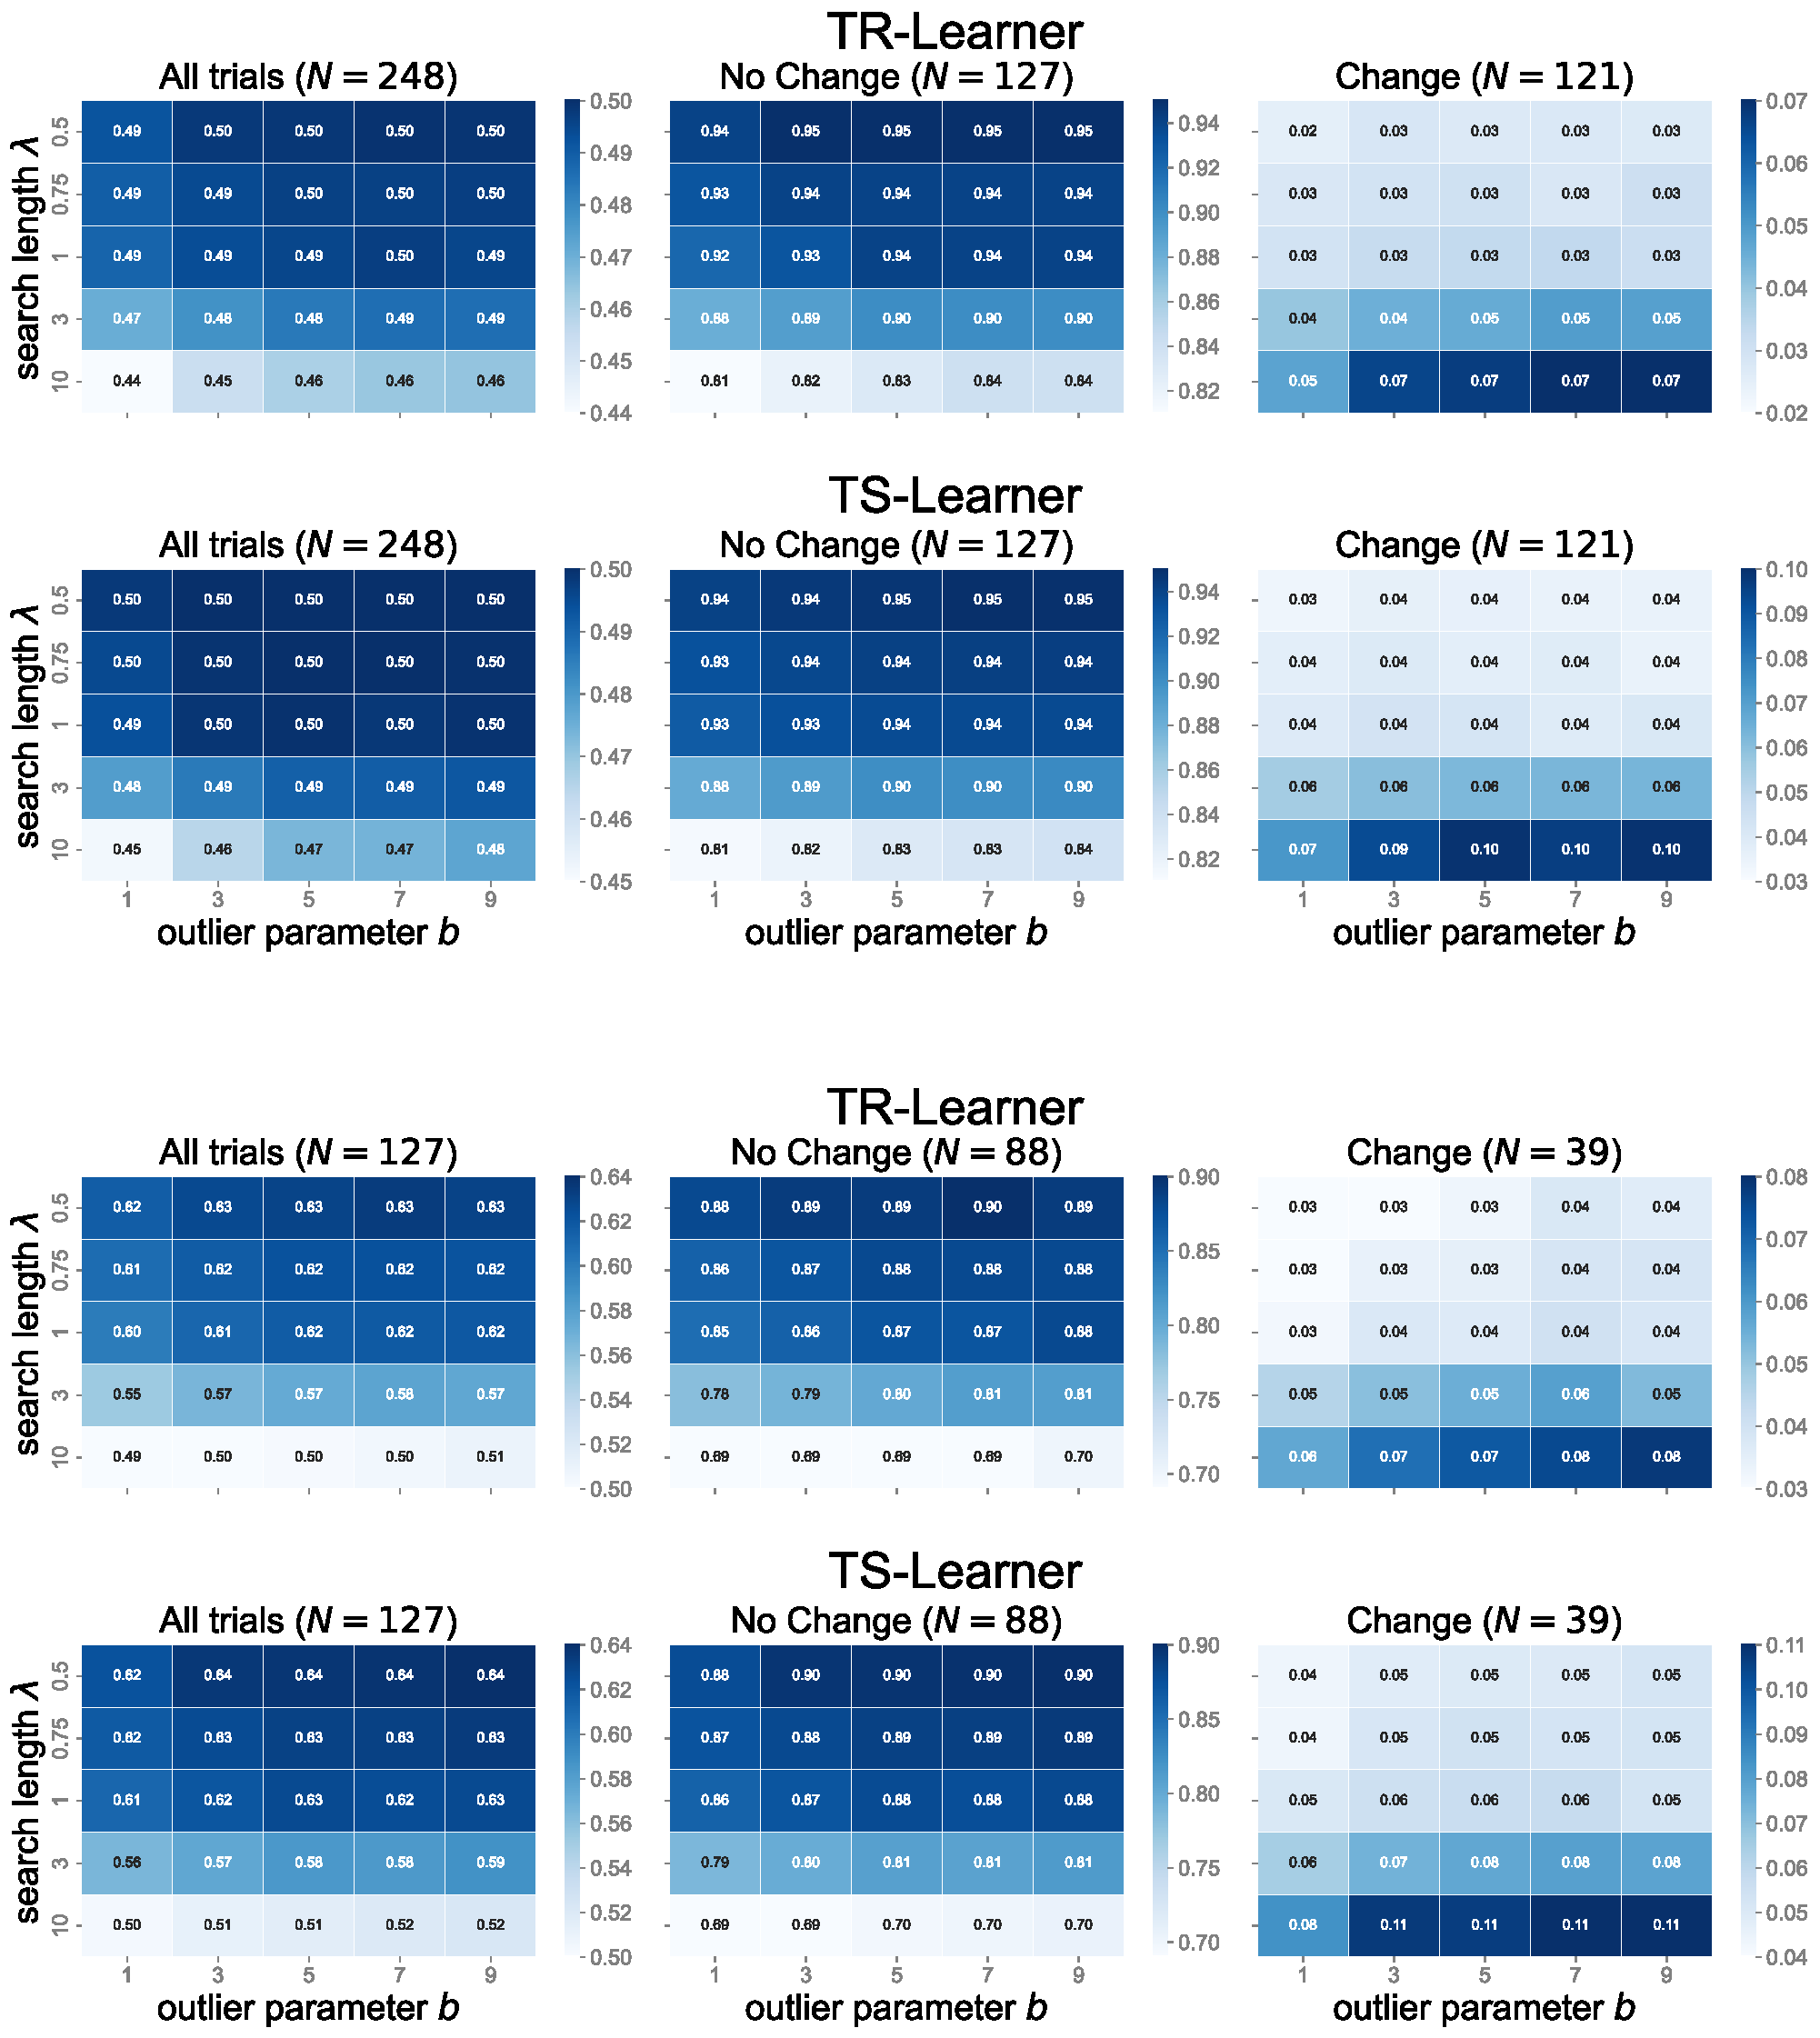
\includegraphics[width=.8\textwidth]{img/fig_8_tr_ts_h_rev.pdf}};
    \draw (-0.25,13.5) node[below] {\textbf{$\mathsf{a)}$}};
    \draw (-0.25,6.3) node[below] {\textbf{$\mathsf{b)}$}};
    \end{tikzpicture}
    \end{center}
    \caption{a) Experiment 1. b) Experiment 2. Both panels show mean likelihood of $\hr$ (shading, darker = more likely) for different values of $\lambda$ and $b$. ``No Change'' subsets out trials during which participants did retain their initial guess (i.e., $\hi$ = $\hr$), ``Change'' subsets trials where $\hi\neq\hr$.
    }
    \label{fig:fig_8_tr_ts_h_rev}
\end{figure*}

\subsection{Predicting generalizations}

Having considered a range of models of the generation of $\hr$, we finally consider whether $\hr$, or adaptive search more generally, can explain participants' generalizations. While we considered end-to-end versions of all the models we compare above, we also considered $\hi$ and $\hr$ as potentially directly predicting participants' generalizations. Consistent with our general thesis that inductive generalizations are driven by learners' symbolic belief about the rule, $\hr$ was by far the single best predictor of revised generalizations across both experiments. See Appendix~A-8 and Table~\ref{table:table_a8_1_generalizations} for details. 


\section{General Discussion}

We explored how people learn symbolic rules in a challenging inductive learning task that admits a practically unbounded compositional hypothesis space. We specifically focused on the relationship between participants’ initial and revised guesses about a hidden symbolic rule. We elicited free text guesses as well as generalizations of predictions to a set of new scenes. Across two experiments, we examined the difference between participants' initial and revised guesses asking whether we can account for these as the result of adaptive search under limited computational capacity. 

Overall, accuracy was close to that which would be expected under posterior sampling or probability matching. However, participants explicit rule guesses were also more complex and less able to account for all the learning data than posterior samples on average. Further diverging from a normative account, we found that participants' revised hypotheses were anchored to their initial hypotheses, containing a much larger overlap of syntactic elements than would be expected under independent sampling or an all-or-none approach like Win--Stay, Lose--Sample. We speculated this could be due to participants considering a short sequence of local edits to their initial hypotheses in the light of new evidence.

To capture participants' guesses in this scheme, we encoded them in lambda calculus and proposed that updated hypotheses were discovered through a short MCMC-like search in which local edits are proposed and accepted according to a fitness function combining prior probability and fit to evidence. We compared an established MCMC proposal distribution (Tree Regrowth) with a stickier variant (Tree Surgery) and compared this account against a set of competitors and benchmarks. We found participants' judgments lined up closest with our Tree-Surgery model in both experiments, suggesting they considered a small number of ``surgical'' elements that replaced part of their earlier guess while minimally disturbing the rest of their rule structure.

\subsection{Search and Positive Testing}
Participants' self-generated tests in phase two of Experiment 1 were subject to a positive testing bias, being much more likely than chance to be rule following under their initial rule guess $\hi$. In Experiment 2, phase two introduced learning data from another participant, presumably driven by confirmation of some other hypothesis not yet considered by the learner. At the same time, participants adapted their guesses more in Experiment 1 and improved in accuracy in Experiment 1 but not Experiment 2. We think a compelling explanation for this pattern is that learners' selected what scenes to test in order to distinguish between their current hypothesis and local alternatives that occurred to them, so actively supporting a process of incremental search of the sort captured by our TR and TS models. Since another person's learning data is less likely to be diagnostic about \emph{these particular} local alternatives, learners in Experiment 2 were less able to use it to adapt and improve their guesses.

While we find this explanation satisfying, we cannot rule out the possibility that yoked learners in Experiment 2 performed worse in phase two than participants in Experiment 1 because they did not process the additional evidence as deeply as they would have had they gathered it themselves trial-by-trial \citep{ruggeri2016active}. Another complicating factor in Experiment 2 could be that participants may have tried to use theory of mind inference, for instance trying to reverse engineer their partner's guess from their testing patterns. This is a notoriously complex problem in general \citep{wu2021representational, shafto2012learning,jara2016naive,hawthorne2019reasoning, wu2021representational}, and perhaps especially challenging in this context since there are numerous ways to test any hypothesis. Nevertheless, social reasoning may still be responsible for some idea generation in the second half of Experiment 2 albeit not to the extent that it allowed participants to perform better than when collecting data themselves. 

\subsection{Limitations and Further Work}
Local search is an important aspect of higher level cognition \citep{hart2020creative, hills2008search, hills2015exploration}. Here, we attempted to reverse engineer people's likely sequences of mental search steps as they grappled with a challenging inductive learning task. While our analyses go significantly beyond past work, our analyses are limited in a number of respects. First, we elicited explicit rule guesses and generalizations after completion of each learning phase, that is, after participants gathered a set of learning data. To allow for a more granular investigation of incremental hypothesis revision over time, future extensions of our work might focus on a learning setting in which learners provide explicit rule guesses after each individual data point. This would unlock the possibility of a closer exploration of how hypotheses shift scene by scene, and how this may relate to the process of active scene construction.

One central assumption of our local adaptation proposal was that people build and edit a single focal hypothesis during compositional inference rather than simultaneously considering many possibilities. Although our analysis showed participants' responses were sequentially dependent, there were cases where participants' responses changed completely. This could mean that people entertain more than one option and are able to switch when one starts to outperform the other. People might also sometimes consider their current candidate to be a ``dead end'' and generate a new hypothesis from scratch \citep{speekenbrink2010learning}. A model that allowed learners to have several hypotheses or ``particles'' in play at a time could help to capture these patterns but is beyond the scope of this project \citep{daw2008pigeon,sanborn2010rational}.

A third limitation is that the present anchoring between $\hi$ and $\hr$ does not necessarily implicate a causal role of the initial rule guess $\hi$. It could also be a consequence of primacy, for instance if a participant only attends to the first few scenes. It might also reflect an incomplete processing of all the evidence, as focusing on only a subset of the potentially relevant features or relations. Such factors might lead to similarity between hypotheses over and above that which is normatively justified by the data but not because the later hypothesis is adapted from the first. This might provide an alternative explanation for why the TS-Learner, which naturally produces the strongest dependence between initial rule guesses ($\hi$) and revised rule guesses ($\hr$) for the same search length was the best predictor of $\hr$. We do not find this explanation particularly compelling, for one because we considered a range of search length values, and also because recency could also result in the opposite pattern, with $\hr$ resulting in too little resemblance to $\hi$. Finally, an incomplete focus on the features would be expected to produce similarity across all judgments, not just those within a learning problem which we did not see.

Investigating how participants generated their initial guesses in the first instance is another interesting question for further research. Specifically, while our PCFG framework provides a recipe for generating hypotheses a priori, it is inherently inefficient and a computationally implausible account of top-down hypothesis generation. Here, we refer to recent work using an instance driven approach to generation \citep{bramley2018grounding}, which suggests that patterns in observed environmental features might directly inspire the generation of new hypotheses that could then be refined and adapted through a local search process such as the one described in the present work. Further contrasting the present learning architectures with alternative models of human concept learning such as the generalization and exemplar learning algorithm SEQL \citep{kuehne2000seql, skorstad1988abstraction} or ALIGN \citep{mclure2010learning} could be another interesting avenue for further work. 

Finally, we note that sample-based approaches represent just one family of approximation to intractable probabilistic inference problems. Variational approaches, that convert inference to an optimisation over some approximation family, have also been explored in a number of recent treatments of bounded cognitive computation. Future work could try to pit variational and sample based approximation against one another as competing accounts of symbolic concept induction \citep{sanborn2017types}.


\subsection{Alternative Representations}
In the present work, we had participants describe their rule guesses in natural language and then translated them into first order logic with references to features of the scenes. As such, we assumed that learners intuitively represent their concepts symbolically and
in terms of the of features and relations we included in our grammar. However, not all concepts are expressible in logic, and statistical concepts are hard to express in natural language. Subsymbolic feature-similarity based representations such as those of exemplar or prototype models might provide an alternative approach to predicting participants' generalizations in the present learning problem \citep{medin1978context,nosofsky1986attention,rosch1999principles}. On that view, linguistic descriptions of reasoning processes might taken to be ``retrospective confabulations'' primarily serving communication rather than capturing the underlying representation \citep{dennett1981making}.  
However, these accounts provide no explanation for how participants readily generated an explicit, symbolically structured rule guess when asked to do so. Additionally, the finding that participants' revised rule guesses were the single best predictor of their generalizations suggests that the simplest explanation for both the guesses and the generalizations is that the guesses drove the generalizations. 

\subsection{Beyond Rule Complexity and Fit}
We modeled inductive inference as a form of program induction. That is, we assumed that participants beliefs progressed via a process involving construction and adaptation of programs (here, ``rules'') guided by their ability to explain data \citep{flener2008introduction, rule2018learning}. While program induction is proving to be a powerful framework for synthesizing human-like concept generation \citep{goodman2008rational, lewis2014error, piantadosi2016logical,lake2015human} and other learning domains \citep{ullman2012theory, rothe2017question, yang2022one}, it is computationally intensive and serves to highlight how tough some of the inference problems solved by humans really are \citep{ullman2012theory}. As such, it seems likely that individual humans chart incomplete paths through such learning settings, employing various hacks, inductive biases, heuristics and approximations along the way \citep{rule2020child}. We see local adaptation as a critical part of this picture, but also note that the perspective invites consideration of other mechanisms for bootstrapping and active search with concomitant cognitive parameters such as motivation and curiosity alongside the search capacity we highlight here. 

\subsection{Conclusions}
The present paper explored the idea that human inductive inference involves adaptation of symbolic hypotheses via sequential local changes in the light of evidence. Across two experiments that varied the source of learners' evidence, we showed a local adaptation mechanism provided a better account of participants’ hypothesis revisions than a set of benchmarks and competitors.  We extend on previous work that explored local adaptation in the large but finite space of causal graphs \citep{bramley2017formalizing} by studying inferences in a setting with an essentially infinite compositional theory space. Moreover, by examining self-generated and yoked learning side by side, we were able to implicate confirmatory testing as potentially subserving a process of local adaptation. Overall, our results suggest that people deal with the inherent complexity of concept inference in part through use of compositional local search.

\subsection{Acknowledgements}
This research was supported by an EPSRC New Investigator Grant (EP/T033967/1) to NRB. JPF acknowledges support from the German Academic Scholarship Foundation. Thanks to Bonan Zhao for help with coding free text responses.

\newcommand{\commiturl}{\url{https://github.com/janphilippfranken/zendo_final_git/\commithash}}
\subsection{Data and Code Availability}
Data and code are available on GitHub at \MYhref{https://github.com/janphilippfranken/FrankenBramleyTheodoropoulos_2022}{FrankenTheodoropoulosBramley2022}. 


\bibliographystyle{apacite}
\bibliography{refs}

\begin{appendices}

\renewcommand{\theequation}{A-\arabic{equation}}
\renewcommand{\thetable}{A-\arabic{table}}
\renewcommand{\thefigure}{A-\arabic{figure}}

% redefine the command that creates the equation no.
\setcounter{equation}{0} % reset counter
\setcounter{table}{0} % reset counter
\setcounter{figure}{0} % reset counter

\section{Appendix}

Appendix~A-1 and Appendix~A-2 provide further technical details on the production process and computation of prior rule generation probabilities. Details of the MCMC approximation scheme and implementation of ``Tree Regrowth'' and ``Tree Surgery'' are provided in Appendix~A-3 and Appendix~A-4. Appendices~A-5--A-7 provide details on our implementation of RULEX, the free response coding scheme used to translate participants' written rule guesses into symbolic rules, and the computation of conditional rule changes. Additional modeling details and supplementary results are provided in Appendix~A-8.

\subsection{A-1: Production Process}\label{ap:a1_production_process}

In our production process, a hypothesis starts with a single \emph{nonterminal} symbol $S$.  We use capital letters as non-terminal symbols. Each production rule replaces a non-terminal symbol with one of the options written in the requisite row of Table~\ref{table:table_a1_1_productions}. The process continues until no non-terminal symbols remain. We assume for simplicity that all possible rewrites are equally probable with the exception of feature selections and value expansions (see Appendix~A-2). For example, since there are three possible expansions for \(S\) each could be selected with probability \(\frac{1}{3}\). The string resulting from this process is guaranteed to be a grammatical statement asserting something about the rule following scenes. Branching resulting from the $A$ and $B$ rewrites can result in an arbitrary number of nested Boolean functions and other complex relationships\footnote{In the present work, we limit the number of quantifiers to 3 for computational convenience.}. For example, the hypothesis \(\exists(\lambda x_{1}: \text{=}(x_{1},small,size), \xx)\) (``there is a small cone'') is produced by the following sequence of productions:

\begin{enumerate}
    \item \(S\) \(\rightarrow\) \(\exists(\lambda x_{1}: A,\xx\))
    \item \(\exists(\lambda x_{1}: A,\xx\)) \(\rightarrow\) \(\exists(\lambda x_{1}: B,\xx\))
    \item \(\exists(\lambda x_{1}: B,\xx\)) \(\rightarrow\) \(\exists(\lambda x_{1}: D,\xx\))
    \item \(\exists(\lambda x_{1}: D,\xx\)) \(\rightarrow\) \(\exists(\lambda x_{1}:  \text{=}(x_1,G),\xx\))
    \item \(\exists(\lambda x_{1}:  \text{=}(x_1,G),\xx\)) \(\rightarrow\) \(\exists(\lambda x_{1}\text{: }  \text{=}(x_1,small,size),\xx\)).
\end{enumerate}


The (syntactic) prior generation probability of the hypothesis (Equation~ \ref{equ:equ_2_prior}) is given by the product of each of the productions that went into creating it: 


\begin{equation}
    \frac{1}{3}\times\frac{1}{2}\times\frac{1}{3}\times  \frac{1}{5} \times \tau_{\mathrm{size}}= \frac{\tau_{\mathrm{size}}}{90}
\label{equ:equ_a1_1_prior_example}
\end{equation}

where $\tau$ refers to the product of the probabilities for feature selection $size$ and value expansion $small$.  


\begin{table}[H]
\centering
\caption{Prior Production Process}
\scriptsize{
\begin{tabular}{llcccccc}
\toprule
Productions\\
\midrule
Start & $S\rightarrow$ & $\exists(\lambda\!x_i\!:~A,\xx)$ & $\forall(\lambda\!x_i\!:~A,\xx)$ & 
$N(\lambda\!x_i\!:~A, K,\xx)$\\
Bind additional & $A\rightarrow$ & B & S\\
Expand & $B\rightarrow$ & D & $C(B,B)$ & $\neg(B)$ \\
% & & .80 & .001 & .20\\  
Function & $D\rightarrow$ &  $I(x_i, E)$ & $I(x_i,x_j,F)$ & $=\!(x_i, G)$ & $=\!(x_i, x_j, H)$ & $\Gamma(x_i, x_j,J)$ \\
Numeric feature & $E\rightarrow$ & value, & feature\\
Numeric feature & $F\rightarrow$ & value, & feature\\
Feature & $G\rightarrow$ & value, & feature\\
Feature & $H\rightarrow$ & value, & feature\\
Relation & $H\rightarrow$ & feature\\
Boolean & $C\rightarrow$ & $\land$ & $\lor$\\
Inequality & $I\rightarrow$ & $\leq$ & $\geq$ & $>$ & $<$\\
Quantifier & $N\rightarrow$ & $\leq$ & $\geq$ & $=$ \\
Number & $K\rightarrow$ & $n\in\{1,2,3\}$\\
\bottomrule
\end{tabular}
\label{table:table_a1_1_productions}

\raggedright Note: Context-sensitive aspects of the grammar: Bound variable(s) sampled uniformly without replacement from set; expressions requiring multiple variables censored if only one. 
}
\end{table}

As there exists and infinite amount of possibilities for realizing a semantic in syntax, we used a rule's estimated semantic generation probability in our analysis instead of working with the syntactic prior. This was given by fitting $\kappa$ in the following function

\begin{equation}
    P(\mathrm{Deriv}_{\mathrm{h-semantic}}) = P(\mathrm{Deriv}_{h}\mid\mathcal{G},\tau)^{\kappa}
\label{equ:equ_a1_2_kappa}
\end{equation}

to a large sample of $N$ synthetic rules in which syntactically distinct rules were clustered based on their meaning (i.e., semantics), and then dividing the size of each cluster by the total size of the synthetic sample. The semantic complexity (cluster size / total size of synthetic sample) was then compared against the median syntactic complexity $P(Deriv_{h}\mid\mathcal{G},\tau)$ from each cluster. Figure~\ref{fig:fig_a1_1_semantic_deriv_prob} illustrates the relationship between a cluster's median log complexity / log prior generation probability (x-axis) and the estimated log semantic generation probability for each rule in the cluster (y-axis). In total, we simulated $N$ = 1,000,000 synthetic rules from our grammar, evaluated each rule against 500 test scenes, resulting in 95,912 distinct clusters following grouping of rules that provided the same predictions for the set of test scenes. Fitting Equation~\ref{equ:equ_a1_2_kappa} to the synthetic rule set shown in Figure~\ref{fig:fig_a1_1_semantic_deriv_prob} resulted in $\kappa$ =  0.486. 




\begin{figure*}[t]
    \begin{center}
      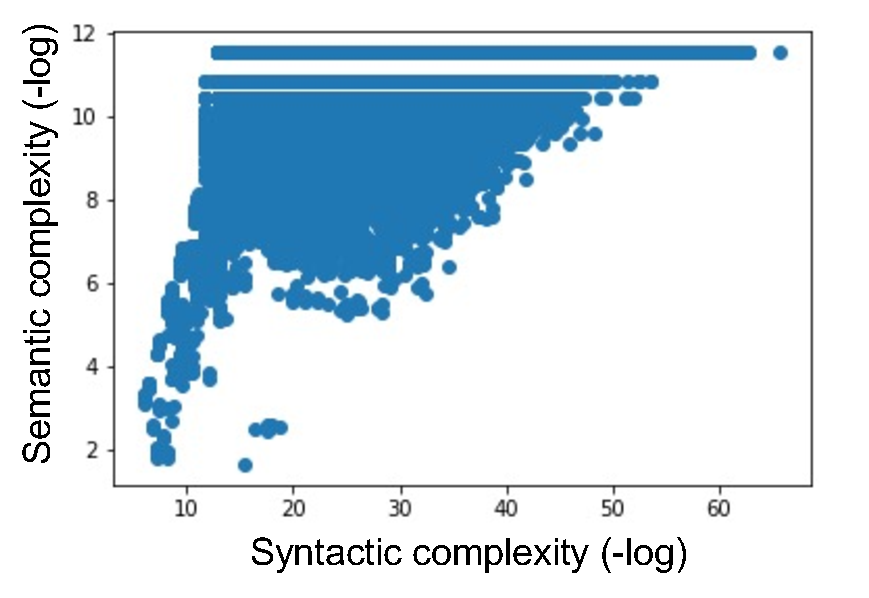
\includegraphics[width=.5\textwidth]{img/fig_a1_semantic_deriv_prob.pdf}
    \end{center}
    \caption{Relationship between cluster's median syntactic rule complexity (x-axis) and estimated semantic complexity of rules in cluster (y-axis). Data correspond to 95,912 clusters obtained from a sample of 1,000,000 synthetic rules generated from the grammar.}
    \label{fig:fig_a1_1_semantic_deriv_prob}
\end{figure*}



\subsection{A-2: Value and Feature Weights}\label{ap:a2_value_and_feat_weights}

In this section, we outline the derivation of production weights for values and features. In previous work \citep{bramley2018grounding}, feature values were sampled uniformly from their support. For example, the values of the feature  $color$ \(\in\) $\{\text{red, blue, green}\}$ would be sampled with probabilities \(\phi_{color}\) = \([\frac{1}{3},\frac{1}{3},\frac{1}{3}]\). For each feature \(i\), the specific feature values \(\textbf{v}_{i}\) thus follow a multinomial distribution \(\textbf{v}_{i}\) $\sim$ Mult(\(n_{i}\), \(\phi_{i}\)) where \(n_{i}\) refers to the number of value expansions for feature $i$ (e.g., \(n_{color}\) = 3 given \(\textbf{v}_{color}\) = $\{\text{red, blue, green}\}$). In our modeling analysis, we weighted value expansion probabilities for each feature based on the content and selections of the scenes generated by the learner during the training phase, whose labels are thus known.

For each feature \(i\), we thus counted the number of occurrences of values \(\textbf{v}_{i}\) between the average rule following scene and the average non-rule following scene. For example, the average rule following scene might include 2.3 red cones, while the average non-rule following scene might include 0 red cones given a hypothesis such as \(\exists(\lambda x_{1}: \text{=}(x_{1},red,color), X)\) (``there is a red one''). The value expansion \(j\) [red] of feature \(i\) [color] thus receives a weight of 2.3. Formally, the score for all specific feature values \(v_{ij}\) is calculated as follows:

\begin{equation}
    v_{ij} =  \frac{1}{|S||r|}\sum_{k = 1, v_{i} \in S||r}^{|v_{i}|} {I}_{v\textsubscript{$ij$}}(x_{k}) -  \frac{1}{|S||\neg r|}\sum_{k = 1, v_{i} \in S||\neg r}^{|v_{i}|}{I}_{v\textsubscript{$ij$}}(x_{k}).
\label{equ:equ_a2_1_value_score}
\end{equation}


Here, \({I}_{v\textsubscript{$ij$}}(x_{k})\) is an indicator function returning 1 if the value of cone \(x_{k}\) is equal to feature value \(v_{ij}\). \(S||r\) refers to the set of test scenes consistent with a rule while \(S||\neg r\) refers to the set of test scenes not consistent with a rule. Importantly, the above equation only accounts for positive influences of feature values on eliciting rule-following scenes (e.g., if the rule was ``there is a red cone'', it would assign higher scores towards the generation of rules mentioning red cones than cones of another color). However, there might be instances in which the absence of a specific feature is critical to a rule. Consider for example the rule ``no cone is upright''. In this case, a scene belongs to the set of rule following scenes \(S||r\) if no cone object is standing upright, meaning that Equation~\ref{equ:equ_a2_1_value_score} might result in a negative value for \(v_{ij}\). To address this issue, the learning procedure is sensitive to the presence \textit{and} absence of features, flipping the value of \(v_{ij}\) if there is no cone \(x_{k}\) that is equal to \(v_{ij}\) in the set of rule following scenes: 


\begin{equation}
    v_{ij} = \begin{cases}
    v_{ij}  \text{ if }\sum_{k = 1, v_{i} \in S||r}^{|v_{i}|}{I}_{v\textsubscript{$ij$}}(x_{k}) > 0\\
    -v_{ij}  \text{ if }\sum_{k = 1, v_{i} \in S||r}^{|v_{i}|}{I}_{v\textsubscript{$ij$}}(x_{k}) = 0. 
    \end{cases}
\label{equ:equ_a2_2_value_score_2}
\end{equation}

Having computed values for each \(v_{ij}\) we add \(\frac{1}{n_{i}}\) to each  \(v_{ij}\) (initial uniform weight prior to observing scenes) and then renormalize scores such that each \(\phi_{i}\) =  \(\sum_{j=1}^{n\textsubscript{i}} v_{ij} = 1\). To determine the relevance of each feature \(i\) on its own, we further weighted the vector over feature probabilities \textbf{\(\psi\)}. Specifically, the probability $\phi$ of sampling a feature $i$ was given by the normalised difference between the feature's value with the highest probability and the feature's value with the lowest probability:


\begin{equation}
    \psi_{i} = \max(\phi_{i}) - \min(\phi_{i}).
\label{equ:equ_a2_3_feat_score}
\end{equation}

That way, production probabilities were ``inherited'' from value to feature level. We added \(\frac{1}{n}\) to each  \(\psi_{i}\) where \(n\) refers to the number of features used in the present task. Finally \(\psi\) was renormalized such that \(\psi\) =  \(\sum_{i=1}^{n}\psi_{i} = 1\).

 
\subsection{A-3: Inference with Tree Regrowth MCMC}\label{ap:a3_inference}

We used Tree Regrowth MCMC also referred to as the ``Rational Rules Model'' \citep{goodman2008rational} with long chains (10,000 samples per chain) to generate normative posterior samples. At each iteration of this approximation, a non-terminal node \(n\) of the current hypothesis \(h\) is selected and deleted. Tree Regrowth then removes all branches below \(n\) and regrowths the tree below \(n\) according to the same stochastic rules used to derive the initial hypothesis \(h\). The probability \(r\) that a new proposal \(h^{'}\) replaces $h$ at the next time step is then given by:

\begin{equation} 
    r = \text{min}(1, \frac{P(D \mid h^{'},b)}{P(D\mid h,b)} \times \frac{P(h^{'}\mid\mathcal{G},\tau)}{P(h\mid\mathcal{G},\tau)}).
\label{equ:equ_a3_1_mcmc}
\end{equation}

At each step of the iteration, proposal \(h^{'}\) is accepted if \(r\) > \(x\) $\leftarrow$ \(\text{Uniform}\)(0,1). If a proposal is rejected, the current hypothesis is retained \(h_{t+1} = h\). 


\subsection{A-4: Tree Surgery as an alternative MCMC proposal distribution}\label{ap:a4_ts_details}
The TR-Learner uses the same established Tree Regrowth mechanism to adapt $\hi$ that we used to generate normative posterior samples (see Appendix~A-3). The difference between normative posterior samples and TR is that TR uses short chains (length parameterised by $\lambda$) that are seeded with $\hi$. This section provides further details on the algorithmic implementation of the TS-Learner shown in Figure~\ref{fig:fig_3_adaptation}b which uses an alternative proposal distribution to adapt $\hi$. Compared to the more mobile TR-Learner, TS retains rule elements when resampling alternatives, thus promoting more local or ``surgical'' edits to a hypothesis. As an example, consider an initial rule \(\hi\): \(\exists(\lambda x_{1}: \text{=}(x_{1},red,color), X)\). After translating this rule into a list-like representation, we get: 

\begin{equation}
    [\exists,[\lambda x_{1}:,=,[x_{1},red,color],X]].
\label{equ:equ_a4_1_ts_1}
\end{equation}

We can extract all non-terminal and terminal productions from this rule recursively: 

\begin{equation}
    \mathrm{productions} = [S,A,B,D,=\!(x_i, G),red,color].
\label{equ:equ_a4_2_ts_2}
\end{equation}

The TS-Learner now targets a random non-terminal in \(n\) \(\in\) \{$S,A,B,D$\} present in $\hi$. The selected non-terminal is replaced with a random proposal from the set of available productions \(\in \mathcal{G}\). For example, the TS-Learner could pick \(S\) and resample the random proposal \(\forall\). The TS-Learner then replaces the initial \(\exists\) with the newly generated proposal, and after transforming the list back into the initial rule representation we get: 

\begin{equation}
    \forall(\lambda x_{1} : \text{=}(x_{1}, red,color),X).
\label{equ:equ_a4_3_ts_3}
\end{equation}

In the above example, the TS-Learner preserves all parts of \(\hi\) except for the quantifier \(\exists\), while the TR-Learner would have resampled all components of the hypothesis following the quantifier, thus increasing the chance of arriving at a very different hypothesis (see also Figure~\ref{fig:fig_3_adaptation}b). The TS-Learner can also apply more complex edits to an initial hypothesis that involve sampling of additional features and values not present in the initial hypothesis \(\hi\). For example, if the TS-Learner targets the non-terminal \(B\) from the set of available non-terminals, we might resample the expansion \(C(B,B)\). After running \(\mathcal{G}\), the TS-Learner might then come up with a new proposal \(h^{'}\) of the form:

\begin{equation}
     \exists(\lambda x_{1}\text{: }  \wedge(\text{=}(x_{1},small,size),\text{=}(x_{1},upright,orientation)), X)
\label{equ:equ_a4_4_ts_4}
\end{equation} 

where \(C\) \(\rightarrow\) \(\wedge\) and the additional \(B\) \(\rightarrow\) \(D\) \(\rightarrow\) \(\text{=}(x_i, G)\) \(\rightarrow\) (\(x1,size\)) \(\rightarrow\) (\(x1,small, size\)). Involving a conjunction during adaptation while maintaining the initial components of $\hi$ is another demonstration of the TS-Learner's emphasis on resolving local uncertainty. A current limitation of our TS-approach is that it did not allow for changes in the number quantifiers resulting from a selection of $A$. In this case, the  TS-Learner followed the same steps as the TR-Learner. 

\subsection{A-5: Our RULEX Implementation}\label{ap:a5_rulex_details}
RULEX traditionally has nine parameters: a lower bound $\lambda$ (minimum number of steps a rule is maintained as long as its performance is above lax criterion $\Phi_L$), an upper bound $\mu$ (maximum number of steps a rule is maintained as long as its performance is above lax criterion $\Phi_L$), lax or performance criterion $\Phi_L$ (minimum proportion of correct classifications required by rule), imperfect acceptance criterion $\Phi_I$ (determines whether a simple rule surviving upper bound $\mu$ is accepted permanently), a conjunctive acceptance criterion $\Phi_C$ (determines whether a conjunctive rule surviving upper bound $\mu$ is accepted permanently), a branching probability $\beta$ (determines probability with which RULEX continues with either imperfect or conjunctive search following incorrect classification of a data point during exact search), storage probability $\sigma$, capacity parameter $\gamma$ ($\sigma$ and $\gamma$ are responsible for computing the probability of storing a current rule), and decision error $\epsilon$ (probability with which a rule makes the opposite response, thus making it probabilistic). Further details on parameter definitions can be found in \cite{navarro2005analyzing}. Fitting the majority of these parameters is not feasible in the current context, since we are forced to use brute force sampling to estimate likelihoods of particular guesses and marginal likelihoods of particular generalizations. Thus we endeavored to somewhat simplify the original RULEX procedure and to use default or previously supported values wherever possible. We here set $\beta$ to 0.5, meaning that our RULEX (referred to as RULEX*) has equal chance of moving to imperfect or conjunct-disjunct search if exact search fails. For both imperfect and conjunct-disjunct search, we set the lower bound to $\lambda$ = 0, meaning that a rule generated by either imperfect or conjunct-disjunct search was disregarded immediately if its performance was below the lax criterion $\Phi_L$ which was initially set to 1 (i.e., a maximum of one incorrect classifications of the 16 training scenes). Once a rule met the requirements of the lax criterion, RULEX* adopts the rule permanently (i.e., $\mu$ = 1) with perfect memory (i.e., $\sigma$ = 1 and $\gamma$ = 1). This means that all \textit{accepted} rules generated during search are stored. If at the imprecise search stage, no rule meets the current lax criterion, we gradually increased the number of accepted incorrect classifications (i.e., updating the lax criterion up to to a maximum of 16 incorrect classifications), repeating either imperfect or conjunct-disjunct search with $\beta$ = 0.5. For simplicity, we set the decision error $\epsilon$ for each single rule guess to zero. We note that our resultant rule predictions are still probabilistic as we average 10,000 sampled RULEX* runs to obtain marginal likelihooods of guesses and generalizations.


\subsection{A-6: Coding Free Responses}\label{ap:a6_free_response_coding}
Natural language free responses were systematically translated into lambda abstraction representations by identifying rule elements and rearranging them into the lambda abstraction format. For a concrete example of a free-text response, consider the guess ``A blue triangle makes Iota waves'' provided by a random participant from Experiment 1. This rule can be translated into the lambda abstraction representation format by identifying the quantifier ``A blue triangle'' \(\rightarrow\) \(\exists\), checking the number of bound variables (one bound variable), identifying  Booleans and equalities (no Booleans, one equality: ``blue triangle'' \(\rightarrow\) ''triangle \(=\) blue''), and finally, features (``color'') and values (``blue''). The resulting lambda representation is then: \(\exists(\lambda x_{1}: \text{=}(x_{1},blue,color), X)\). Importantly, the order in which participants entered rules was preserved during translation, meaning that two semantically equivalent rules (``there is a small red'', ``there is a red that is small'') resulted in two syntactically different structures to match participants' free responses as closely as possible. In our grammar, we only included a single relational operator (``contact''). However, other potential relational operators were identified during encoding of free responses (e.g., ``stacked'' or ``pointing at each other''). Rules including such operators were excluded from our analysis, which primarily focused on non-relational operators. If participants provided multiple rules for a trial, we used their first rule in our analysis (this happened in less than <5\% of trials). Finally, when translating quantifiers, we looked for words such as ``one’’ or ‘’two’’. If participants wrote e.g., ``just a single red’’, this would have resulted in the same translated rule as ``there needs to be one red''. All rules and translated responses have been uploaded to GitHub.


\subsection{A-7: Conditional Change Probabilities}\label{ap:a7_conditional_change_probabilities}
We expected the probability with which participants changed rule elements (quantifiers, Booleans, equalities, features, values) given a change to a specific element (e.g., quantifier change) to be smaller compared to the probability with which rule elements were changed between initial and revised posterior samples. As an example of how we calculated conditional change probabilities, consider a change in quantifiers from ``exists'' to ``exactly'' (e.g., ``there is a red'' $\rightarrow$ ``there is exactly one red''). In this example, the root of the hypothesis tree, the quantifier, changed. However, references to the color feature and value red are retained therefore there are no conditional changes in feature and value, and no opportunity for additional changes in Booleans (since there are none) or quantifiers (since the only one was changed already). On the other hand, going from ``there is a blue'' to a revised guess of ``there is exactly one large red'' involves considerably more changes. Conditioning on the quantification change, we now see that additionally the color feature value has changed (from blue to red) and several additional elements have been added ($+$1 Boolean, $+$1 equality, $+$1 feature, and $+$1 value). Such additions are shown in the ``Number of Added and Removed Elements'' panel in Figure~\ref{fig:fig_5_exp_1_behavioural_res}e and Figure~\ref{fig:fig_6_exp_2_behavioural_res}e). Several rules included multiple elements of the same class (e.g., two Booleans), which is why the diagonal entries of Figure~\ref{fig:fig_5_exp_1_behavioural_res}d and Figure~\ref{fig:fig_6_exp_2_behavioural_res}d are not equal to 1.0. Diagonal entries reflect the average frequency with which changes to one element result in changes to other elements of the same class. As an example, consider the expression ``one that is small and red lying on its left hand side'' $\rightarrow$ ``one that is small or red lying on its left hand side''. Here, on a minimal change construal, the conjunction ``and'' has changed to the disjunction ``or''. The change probability of Booleans conditional on this change ``and'' $\rightarrow$ ``or'' is thus $\frac{1}{2}$, since one of the two original Booleans has changed ($\{\text{and, and}\} \rightarrow \{\text{or, and}\}$).
 
\subsection{A-8: Additional Modeling Details}\label{ap:8_modeling_details}

\subsubsection{Modeling Generalizations}

We fit all models to predict participants' generalizations using a single a decision noise parameter \(\omega\). Specifically, the probability that participant $p$ selected scene $s$ during trial $t$ as rule following was modeled as the average over a model's softmaxed predictions: 

\begin{equation}
    P(\mathrm{choose}_{pt}=s) = \frac{1}{N}\sum_i^N \frac{e^{P(s)^i_{pt}/\omega}}{e^{P(s)^i_{pt}/\omega} + e^{(1-P(s)^i_{pt})/\omega}}.
\label{equ:equ_a8_1_softmax}
\end{equation}

$\omega\rightarrow 0$ indicates hard maximization over $P(s)$, while $\omega\rightarrow\infty$ indicates random responding. We fit $\omega$ to the full set of responses for all models using maximum likelihood estimation. For generating normative predictions, we again used the posterior predictive distributions over the posterior samples used earlier for analyses. To generate generalization predictions for the TR-Learner and TS-Learner blind to participants' revised rules we ran 1000 independent chains starting from participants' initial rules, each time keeping the final edit. For RULEX*, we computed the average over 10,000 softmaxed rule predictions using the same bag of rules used to predict $\hr$. We further included a random response baseline that has no parameters and simply assigns a 0.5 probability to each generalization selection. Table~\ref{table:table_a8_1_generalizations} shows best fitting results of participants' generalizations\footnote{To generate predictions for the posterior sample, the softmax was applied only once using the average prediction across the 10,000 rules in the sample.}. 

We note that while RULEX* fits generalizations better than TR and TS for both experiments we do not think its win is meaningful since it does so with a minimally small search parameter $\lambda = .5$ meaning it has almost zero chance of generating a better alternative than $\hi$. RULEX* here outperforms $\hi$ by being minimally adaptive, using $\hi$ to make predictions whenever it is consistent with all the learning data or making essentially random predictions otherwise. End to end TR-Learner, TS-Learner and RULEX* accounts all outperform the predictions of independent Posterior Sampled rules or the MAP in predicting the revised generalizations, but do not come close to matching the predictions of the participants' own reported $\hr$.

\begin{table*}[!ht]
\begin{center} 
\caption{Best fitting model performances for participants' revised generalizations (Gen.).} 
\vskip 0.10in
\begin{tabular}{l r c c c c c} 
\small
Experiment & Model & Mean $BIC_{\text{Gen.}}$ & $b$ & $\lambda$ & $\omega$\\ 
\toprule
% exp 1
\multirow{9}{*}{Exp. 1} & $\text{Random Baseline}$ & 11.090 & - & - & $\infty$\\
& $\hi$ & 8.810 & - & - & 0.861\\
& $\mathbf{h}_{\mathrm{\textbf{rev.}}}$ & \textbf{6.777} & - & - & \textbf{0.576}\\
& $\text{Posterior Sample (PS)}$ & 9.144  & 7.0 & - & 0.820\\
& $\text{Maximum a posteriori (MAP)}$ & 9.355  & 9.0 & - & 0.999\\
& $\text{Win--stay, lose--sample (WSLS)}$ & 9.012 & 7.0 & - & 1.189\\
& $\text{WSLS with Tree Regrowth (TR)}$ & 8.407 & 5.0 & 3.0 & 0.636\\
& $\text{WSLS with Tree Surgery (TS)}$ & 8.350 & 5.0 & 3.0 & 0.622\\
& $\text{RULEX}^*$ & 8.272 & - & 0.5 & 0.388\\
\midrule
% exp 2
\multirow{9}{*}{Exp. 2} & $\text{Random Baseline}$ & 11.090 & - & - & $\infty$\\
& $\hi$ & 8.729 & - & - & 0.840\\
& $\mathbf{h}_{\mathrm{\textbf{rev.}}}$ & \textbf{7.862} & - & - & \textbf{0.696}\\
& $\text{Posterior Sample (PS)}$ & 9.469 & 5.0 & - & 0.900\\
& $\text{Maximum a posteriori (MAP)}$ & 9.541 & 7.0 & - & 1.051\\
& $\text{Win--stay, lose--sample (WSLS)}$ & 9.120  & 5.0  & - & 1.236\\
& $\text{WSLS with Tree Regrowth (TR)}$ & 8.437 & 7.0 & 1.0 & 0.653\\
& $\text{WSLS with Tree Surgery (TS)}$ & 8.413  & 9.0 & 0.75 & 0.654\\
& $\text{RULEX}^*$ & 8.268  & - & 0.5 & 0.395\\
\bottomrule
\label{table:table_a8_1_generalizations}
\end{tabular}
\end{center} 
\end{table*}

\subsubsection{Supplementary Modeling Results}

Tables~\ref{table:table_a8_2_exp_1_norm_model_res}-\ref{table:table_a8_7_exp_2_rulex_model_res} include modeling results for each parameter combination of $\lambda$ and $b$ with $\epsilon=\frac{1}{10,000}$ for trials during which a model failed to identify $\hr$. $N_{{\text{Found}}_{\hr}}$ corresponds to the number of trials during which $\hr$ was identified by a model. For example $N_{{\text{Found}}_{\hr}}$ = 134 means that during 134 out of the total 248 trials in Experiment 1, a posterior sample of size 10,000 contained at least one rule semantically identical to $\hr$. ``Gen. Accuracy'' refers to the accuracy of a each model's generalization selections and ``Freq. True Rule'' to the probability of the model guessing the ground truth correctly. We also provide best fitting modeling results for $\hr$ using $\epsilon=\frac{1}{100,000}$ to demonstrate that the ranking of our models was not a function of $\epsilon$. These are shown in Table~\ref{table:table_a8_8_mean_prob_100000k}. As expected, fits for each model are worse as trials in which $\hr$ was not found have now a log probability of $log(\frac{1}{100,000})$ instead of $log(\frac{1}{10,000})$. In our main results (Table~\ref{table:table_4_h_rev}), we use $\epsilon=\frac{1}{10,000}$ as $10,000$ corresponded to the total number of rules simulated by each model during our analysis of $\hr$.
 
\begin{table*}[!ht]
\begin{center} 
\caption{Experiment 1. Normative modeling results for different values of $b$ (248 Trials).} 
\vskip 0.10in
\resizebox{\columnwidth}{!}{
\begin{tabular}{c c c c c c c} 
\small
$b$ & Model & Mean $BIC_{\hr}$ &  $N_{{\text{Found}}_{\hr}}$  & $Mean BIC_{\text{Gen.}}$ & Gen. Accuracy & Freq. True Rule \\ 
\toprule
% b = 1
& $\text{Normative}$ & 11.307 & 134 & 10.941 ($\omega$ = 2.331) & 0.626 & 0.180\\

1 & $\text{MAP}$ & 12.724 & 77 & 10.361 ($\omega$ = 1.568) & 0.755 & 0.403 \\

& $\text{WSLS}$ & 7.158 & 181 & 10.415 ($\omega$ = 2.257) & 0.743 & 0.400\\

\midrule
% b = 3
& $\text{Normative}$ & 10.567 & 121 & 10.000 ($\omega$ = 1.097) & 0.772 & 0.423\\

3 & $\text{MAP}$ & 12.129 & 85 & 10.001 ($\omega$ = 1.280) & 0.810 & 0.488 \\

& $\text{WSLS}$ & 8.809 & 170 & 9.634 ($\omega$ = 1.502) & 0.821 & 0.525\\

\midrule
% b = 5
& $\text{Normative}$ & 9.817 & 127 & 9.434 ($\omega$ = 0.896) & 0.825 & 0.545\\

5 & $\text{MAP}$ & 11.238 & 97 & 9.603 ($\omega$ = 1.086) & 0.842 & 0.589 \\

& $\text{WSLS}$ & 10.058 & 171 & 9.226 ($\omega$ = 1.287) & 0.858 & 0.616\\

\midrule
% % b = 7
& $\text{Normative}$ & 10.037 &  123 & 9.144 ($\omega$ = 0.820) & 0.838 & 0.560\\

7 & $\text{MAP}$ & 11.164 & 98 & 9.363 ($\omega$ = 1.001) & 0.862 & 0.613 \\

& $\text{WSLS}$ & 11.843 & 167 & 9.012 ($\omega$ = 1.189) & 0.866 & 0.627\\

\midrule
% b = 9
& $\text{Normative}$ & 10.244 & 120 & 9.196 ($\omega$ = 0.837) & 0.825 & 0.522\\

9 & $\text{MAP}$ & 11.535 & 93 &  9.355 ($\omega$ = 0.999) & 0.841 & 0.560 \\

& $\text{WSLS}$ & 13.326 & 167 &  9.036 ($\omega$ = 1.202) & 0.858 & 0.601 \\

\bottomrule


\label{table:table_a8_2_exp_1_norm_model_res}
\end{tabular}}
\end{center} 
\end{table*}


\begin{table*}[!ht]
\begin{center} 
\caption{Experiment 1. TR- and TS results for different values of $\lambda$ and $b$ (248 Trials).} 
\vskip 0.10in
\resizebox{\columnwidth}{!}{
\begin{tabular}{c c c c c c c c} 
\small

$\lambda$ & $b$ & Model & $Mean BIC_{\hr}$ &  $N_{{\text{Found}}_{\hr}}$  & Mean $BIC_{\text{Gen.}}$ & Gen. Accuracy & Freq. True Rule \\ 

\toprule
% lam .5
% b = 1
& 1 & $\text{TR}$ & 6.920 & 192 & 8.481 ($\omega$ = 0.651) & 0.710 & 0.326\\
& 1 & $\text{TS}$ & 6.445 & 191 & 8.437 ($\omega$ = 0.646) & 0.711 & 0.329\\
% b = 3
& 3 & $\text{TR}$ & 6.955 & 190 & 8.507 ($\omega$ = 0.685) & 0.714 & 0.327\\
& 3 & $\text{TS}$ & 6.538 & 194 & 8.474 ($\omega$ = 0.677) & 0.715 & 0.330\\
% b = 5
0.5  & 5 & $\text{TR}$ & 7.007 & 190 & 8.508 ($\omega$ = 0.694) & 0.715 & 0.328\\
& 5 & $\text{TS}$ & 6.699 & 186 & 8.479 ($\omega$ = 0.686) & 0.716 & 0.330\\
% % b = 7
& 7 & $\text{TR}$ & 7.113 & 181 & 8.509 ($\omega$ = 0.696) & 0.715 & 0.328\\
& 7 & $\text{TS}$ & 6.701 & 194 & 8.488 ($\omega$ = 0.690) & 0.716 & 0.330\\
% b = 9
& 9 & $\text{TR}$ & 7.158 & 188 & 8.515 ($\omega$ = 0.699) & 0.716 & 0.328\\
& 9 & $\text{TS}$ & 6.638 & 195 & 8.496 ($\omega$ = 0.692) & 0.716 & 0.330\\
\midrule

%  lam 0.75
% b = 1
& 1 & $\text{TR}$ & 6.774 & 194 & 8.448 ($\omega$ = 0.637) & 0.709 & 0.326\\
& 1 & $\text{TS}$ & 6.340 & 194 & 8.405 ($\omega$ = 0.630) & 0.711 & 0.329\\
% b = 3
& 3 & $\text{TR}$ & 6.903 & 193 & 8.470 ($\omega$ = 0.671) & 0.714 & 0.328\\
& 3 & $\text{TS}$ & 6.456 & 196 & 8.452 ($\omega$ = 0.666) & 0.715 & 0.331\\
% b = 5
0.75 & 5 & $\text{TR}$ & 6.943 & 193 & 8.481 ($\omega$ = 0.683) & 0.715 & 0.328\\
& 5 & $\text{TS}$ & 6.584 & 190 & 8.459 ($\omega$ = 0.676) & 0.716 & 0.330\\
% % b = 7
& 7 & $\text{TR}$ & 7.085 & 188 & 8.494 ($\omega$ = 0.688) & 0.716 & 0.328\\
& 7 & $\text{TS}$ & 6.624 & 188 & 8.461 ($\omega$ = 0.679) & 0.716 & 0.331\\
% b = 9
& 9 & $\text{TR}$ & 7.012 & 187 & 8.487 ($\omega$ = 0.688) & 0.716 & 0.329\\
& 9 & $\text{TS}$ & 6.648 & 191 & 8.468 ($\omega$ = 0.680) & 0.717 & 0.331\\

\midrule
% lam 1
% b = 1
& 1 & $\text{TR}$ & 6.794 & 195 &  8.435 ($\omega$ = 0.626) & 0.709 & 0.327\\
& 1 & $\text{TS}$ & 6.244 & 202 &  8.401 ($\omega$ = 0.621) & 0.711 & 0.329\\
% b = 3
& 3 & $\text{TR}$ & 6.834 & 193 &  8.453 ($\omega$ = 0.662) & 0.714 & 0.329\\
& 3 & $\text{TS}$ & 6.372 & 197 &  8.420 ($\omega$ = 0.654) & 0.716 & 0.331\\
% b = 5
1 & 5 & $\text{TR}$ & 6.986 & 190 &  8.464 ($\omega$ = 0.673) & 0.716 & 0.716\\
& 5 & $\text{TS}$ & 6.410 & 192 &  8.433 ($\omega$ = 0.665) & 0.716 & 0.332\\
% % b = 7
& 7 & $\text{TR}$ & 6.972 & 188 &  8.474 ($\omega$ = 0.678) & 0.716 & 0.329\\
& 7 & $\text{TS}$ & 6.541 & 194 &  8.438 ($\omega$ = 0.668) & 0.717 & 0.332\\
% b = 9
& 9 & $\text{TR}$ & 6.964 & 189 &  8.482 ($\omega$ = 0.681) & 0.716 & 0.329\\
& 9 & $\text{TS}$ & 6.551 & 192 &  8.447 ($\omega$ = 0.672) & 0.717 & 0.331\\
\midrule
% lam 3
% b = 1
& 1 & $\text{TR}$ & 6.491 & 197 &  8.453 ($\omega$ = 0.587) & 0.707 & 0.328\\
& 1 & $\text{TS}$ & 5.986 & 200 &  8.378 ($\omega$ = 0.576) & 0.710 & 0.333\\
% b = 3
& 3 & $\text{TR}$ & 6.649 & 200 &  8.437 ($\omega$ = 0.628) & 0.715 & 0.332\\
& 3 & $\text{TS}$ & 5.963 & 201 &  8.366 ($\omega$ = 0.612) & 0.718 & 0.337\\
% b = 5
3 & 5 & $\text{TR}$ & 6.610 & 197 &  8.407 ($\omega$ = 0.636) & 0.718 & 0.333\\
& 5 & $\text{TS}$ & 6.132 & 197 &  8.350 ($\omega$ = 0.622) & 0.720 & 0.338\\
% % b = 7
& 7 & $\text{TR}$ & 6.707 & 191 &  8.411 ($\omega$ = 0.640) & 0.719 & 0.334\\
& 7 & $\text{TS}$ & 6.180 & 196 &  8.371 ($\omega$ = 0.629) & 0.720 & 0.338\\
% b = 9
& 9 & $\text{TR}$ & 6.639 & 195 &  8.399 ($\omega$ = 0.641) & 0.719 & 0.334\\
& 9 & $\text{TS}$ & 6.156 & 196 &  8.353 ($\omega$ = 0.628) & 0.721 & 0.339\\
\midrule
% lam 10
% b = 1
& 1 & $\text{TR}$ & 6.509 & 202 &  8.821 ($\omega$ = 0.610) & 0.705 & 0.331\\
& 1 & $\text{TS}$ & 5.962 & 204 &  8.684 ($\omega$ = 0.576) & 0.708 & 0.336\\
% b = 3
& 3 & $\text{TR}$ & 6.368 & 204 &  8.673 ($\omega$ = 0.636) & 0.719 & 0.341\\
& 3 & $\text{TS}$ & 5.925 & 203 &  8.520 ($\omega$ = 0.597) & 0.723 & 0.350\\
% b = 5
10 & 5 & $\text{TR}$ & 6.504 & 200 &  8.562 ($\omega$ = 0.633) & 0.724 & 0.344\\
& 5 & $\text{TS}$ & 5.917 & 203 &  8.434 ($\omega$ = 0.600) & 0.728 & 0.352\\
% % b = 7
& 7 & $\text{TR}$ & 6.622 & 200 &  8.536 ($\omega$ = 0.633) & 0.725 & 0.345\\
& 7 & $\text{TS}$ & 5.994 & 202 &  8.417 ($\omega$ = 0.604) & 0.729 & 0.353\\
% b = 9
& 9 & $\text{TR}$ & 6.790 & 194 &  8.527 ($\omega$ = 0.635) & 0.726 & 0.345\\
& 9 & $\text{TS}$ & 6.033 & 203 &  8.412 ($\omega$ = 0.606) & 0.730 & 0.354\\
\midrule


\label{table:table_a8_3_exp_1_tr_ts}
\end{tabular}}
\end{center} 
\end{table*}

\begin{table*}[!ht]
\begin{center} 
\caption{Experiment 1. RULEX* results for different values of $\lambda$ (248 Trials).} 
\vskip 0.10in
\resizebox{\columnwidth}{!}{
\begin{tabular}{c c c c c c c} 
\small
$\lambda$ & Model & $Mean BIC_{\hr}$ &  $N_{{\text{Found}}_{\hr}}$  & Mean $BIC_{\text{Gen.}}$ & Gen. Accuracy & Freq. True Rule \\ 
\toprule
0.5 & $\text{RULEX*}$ & 9.964 & 170 & 8.272 ($\omega$ = 0.388) & 0.676 & 0.323 \\
0.75 & $\text{RULEX*}$ & 9.870 & 172 & 8.341 ($\omega$ = 0.394) & 0.677 & 0.323 \\
1 & $\text{RULEX*}$ & 9.811 & 172 & 8.414 ($\omega$ = 0.402) & 0.678 & 0.324 \\
3 & $\text{RULEX*}$ & 9.594 & 168 & 9.001 ($\omega$ = 0.517) & 0.685 & 0.325 \\
10 & $\text{RULEX*}$ & 9.202 & 166 & 9.385 ($\omega$ = 0.693) & 0.698 & 0.328 \\
\bottomrule
\label{table:table_a8_4_exp_1_rulex_model_res}
\end{tabular}}
\end{center} 
\end{table*}

% exp 2
\begin{table*}[!ht]
\begin{center} 
\caption{Experiment 2. Normative results for different values of $b$ (127 Trials).} 
\vskip 0.10in
\resizebox{\columnwidth}{!}{
\begin{tabular}{c c c c c c c} 
\small

$b$ & Model & $Mean BIC_{\hr}$ &  $N_{{\text{Found}}_{\hr}}$  & $Mean BIC_{\text{Gen.}}$ & Gen. Accuracy & Freq. True Rule \\ 
\toprule
% b = 1
& $\text{Normative}$ & 11.782 & 68 & 10.866 ($\omega$ = 1.776) & 0.634 & 0.184\\

1 & $\text{MAP}$ & 13.527 & 34 & 10.349 ($\omega$ = 1.523) & 0.766 & 0.409 \\

& $\text{WSLS}$ & 6.573 & 103 &  10.248 ($\omega$ = 1.932) & 0.744 & 0.367\\

\midrule
% b = 3
& $\text{Normative}$ & 12.027 & 51 &  9.755 ($\omega$ = 0.955) & 0.796 & 0.470\\

3 & $\text{MAP}$ & 12.947 & 38 & 9.687 ($\omega$ = 1.107) & 0.843 & 0.559 \\

& $\text{WSLS}$ & 10.926 & 99 &  9.367 ($\omega$ = 1.329) & 0.832 & 0.532\\

\midrule
% b = 5
& $\text{Normative}$ & 11.403 & 56 &  9.469 ($\omega$ = 0.900) & 0.823 & 0.503\\

5 & $\text{MAP}$ & 12.657 & 40 &  9.571 ($\omega$ = 1.062) & 0.852 & 0.551 \\

& $\text{WSLS}$ & 14.836 & 100 & 9.120 ($\omega$ = 1.236) & 0.844 & 0.557\\

\midrule
% % b = 7
& $\text{Normative}$ & 11.681 & 52 &  9.488 ($\omega$ = 0.923) & 0.837 & 0.554\\

7 & $\text{MAP}$ & 12.367 & 42 &  9.541 ($\omega$ = 1.051) & 0.862 & 0.614 \\

& $\text{WSLS}$ & 19.7401 & 98 &  9.142 ($\omega$ = 1.262) & 0.858 & 0.589 \\

\midrule
% b = 9
& $\text{Normative}$ & 12.340 & 49 & 9.790 ($\omega$ = 1.033) & 0.833 & 0.536\\

9 & $\text{MAP}$ & 13.817 & 32 &  9.866 ($\omega$ = 1.188) & 0.861 & 0.606 \\

& $\text{WSLS}$ & 24.0569 & 97 & 9.314 ($\omega$ = 1.332) & 0.865 & 0.596\\

\bottomrule

\label{table:table_a8_5_exp_2_norm_model_res}
\end{tabular}}
\end{center} 
\end{table*}


\begin{table*}[!ht]
\begin{center} 
\caption{Experiment 2. TR- and TS results for different values of $\lambda$ and $b$ (127 Trials).} 
\vskip 0.10in
\resizebox{\columnwidth}{!}{
\begin{tabular}{c c c c c c c c} 
\small

$\lambda$ & $b$ & Model & $Mean BIC_{\hr}$ &  $N_{{\text{Found}}_{\hr}}$  & Mean $BIC_{\text{Gen.}}$ & Gen. Accuracy & Freq. True Rule \\ 

\toprule
% lam .5
% b = 1
& 1 & $\text{TR}$ & 4.615 & 106 &  8.519 ($\omega$ = 0.650) & 0.713 & 0.286\\
& 1 & $\text{TS}$ & 4.095 & 109 &  8.481 ($\omega$ = 0.647) & 0.715 & 0.288\\
% b = 3
& 3 & $\text{TR}$ & 4.711 & 105 &  8.490 ($\omega$ = 0.667) & 0.716 & 0.287\\
& 3 & $\text{TS}$ & 4.145 & 107 &  8.446 ($\omega$ = 0.658) & 0.718 & 0.289\\
% b = 5
0.5  & 5 & $\text{TR}$ & 4.694 & 107 &  8.471 ($\omega$ = 0.670) & 0.717 & 0.287\\
& 5 & $\text{TS}$ & 4.220 & 106 &  8.453 ($\omega$ = 0.664) & 0.719 & 0.290\\
% % b = 7
& 7 & $\text{TR}$ & 4.671 & 106 &  8.465 ($\omega$ = 0.670) & 0.717 & 0.287\\
& 7 & $\text{TS}$ & 4.271 & 106 &  8.452 ($\omega$ = 0.667) & 0.719 & 0.289\\
% b = 9
& 9 & $\text{TR}$ & 4.752 & 102 &  8.449 ($\omega$ = 0.668) & 0.717 & 0.288\\
& 9 & $\text{TS}$ & 4.252 & 106 &  8.447 ($\omega$ = 0.667) & 0.719 & 0.289\\
\midrule
%  lam 0.75
% b = 1
& 1 & $\text{TR}$ & 4.495 & 107 & 8.510 ($\omega$ = 0.641) &  0.712 & 0.290\\
& 1 & $\text{TS}$ & 4.108 & 109 & 8.463 ($\omega$ = 0.636) & 0.715 & 0.288\\
% b = 3
& 3 & $\text{TR}$ & 4.707 & 106 & 8.472 ($\omega$ = 0.657) &  0.715 & 0.287\\
& 3 & $\text{TS}$ & 4.268 & 106 & 8.437 ($\omega$ = 0.651) &  0.718 & 0.290\\
% b = 5
0.75 & 5 & $\text{TR}$ & 4.657 & 105 & 8.470 ($\omega$ = 0.663) & 0.716 & 0.287\\
& 5 & $\text{TS}$ & 4.250 & 105 & 8.442 ($\omega$ = 0.657) &  0.719 & 0.290\\
% % b = 7
& 7 & $\text{TR}$ & 4.669 & 104 & 8.453 ($\omega$ = 0.662) &  0.720 & 0.287\\
& 7 & $\text{TS}$ & 4.245 & 107 & 8.443 ($\omega$ = 0.659) &  0.719 & 0.290\\
% b = 9
& 9 & $\text{TR}$ & 4.621 & 106 & 8.444 ($\omega$ = 0.661) &  0.717 & 0.288\\
& 9 & $\text{TS}$ & 4.255 & 107 & 8.413 ($\omega$ = 0.654) &  0.720 & 0.291\\
\midrule
% lam 1
% b = 1
& 1 & $\text{TR}$ &4.473 & 110 & 8.506 ($\omega$ = 0.633) & 0.711 & 0.287\\
& 1 & $\text{TS}$ & 4.065 & 110 & 8.461 ($\omega$ = 0.628) & 0.714 & 0.289\\
% b = 3
& 3 & $\text{TR}$ & 4.656 & 108 & 8.475 ($\omega$ = 0.652) & 0.715 & 0.288\\
& 3 & $\text{TS}$ & 4.190 & 108 & 8.447 ($\omega$ = 0.647) & 0.718 & 0.290\\
% b = 5
1 & 5 & $\text{TR}$ & 4.635 & 107 & 8.449 ($\omega$ = 0.653) & 0.716 & 0.288\\
& 5 & $\text{TS}$ & 4.199 & 107 & 8.447 ($\omega$ = 0.652) & 0.719 & 0.291\\
% % b = 7
& 7 & $\text{TR}$ & 4.679 & 105 & 8.437 ($\omega$ = 0.653) & 0.717 & 0.288\\
& 7 & $\text{TS}$ & 4.192 & 106 & 8.442 ($\omega$ = 0.653) & 0.719 & 0.291\\
% b = 9
& 9 & $\text{TR}$ & 4.657 & 106 & 8.441 ($\omega$ = 0.655) & 0.717 & 0.288\\
& 9 & $\text{TS}$ & 4.263 & 105 & 8.420 ($\omega$ = 0.649) & 0.719 & 0.291\\
\midrule
% lam 3
% b = 1
% b = 1
& 1 & $\text{TR}$ & 4.656 & 109 & 8.630 ($\omega$ = 0.620) & 0.707 & 0.289\\
& 1 & $\text{TS}$ & 4.155 & 110 & 8.561 ($\omega$ = 0.609) & 0.711 & 0.292\\
% b = 3
& 3 & $\text{TR}$ & 4.615 & 109 & 8.560 ($\omega$ = 0.641) & 0.713 & 0.291\\
& 3 & $\text{TS}$ & 4.297 & 108 & 8.504 ($\omega$ = 0.627) & 0.717 & 0.296\\
% b = 5
3 & 5 & $\text{TR}$ & 4.650 & 108 & 8.518 ($\omega$ = 0.640) & 0.715 & 0.291\\
& 5 & $\text{TS}$ & 4.316 & 106 & 8.489 ($\omega$ = 0.631) & 0.718 & 0.297\\
% % b = 7
& 7 & $\text{TR}$ & 4.740 & 106 & 8.503 ($\omega$ = 0.639) & 0.716 & 0.292\\
& 7 & $\text{TS}$ & 4.232 & 107 & 8.458 ($\omega$ = 0.628) & 0.719 & 0.297\\
% b = 9
& 9 & $\text{TR}$ & 4.687 & 107 & 8.503 ($\omega$ = 0.643) & 0.716 & 0.291\\
& 9 & $\text{TS}$ & 4.243 & 107 & 8.434 ($\omega$ = 0.628) & 0.719 & 0.297\\
\midrule
% lam 10
% b = 1
& 1 & $\text{TR}$ & 5.209 & 110 & 8.979 ($\omega$ = 0.669) & 0.704 & 0.292\\
& 1 & $\text{TS}$ & 4.781 & 110 & 8.911 ($\omega$ = 0.645) & 0.707 & 0.297\\
% b = 3
& 3 & $\text{TR}$ & 5.495 & 111 & 8.914 ($\omega$ = 0.693) & 0.714 & 0.297\\
& 3 & $\text{TS}$ & 4.963 & 109 & 8.802 ($\omega$ = 0.665) & 0.719 & 0.309\\
% b = 5
10 & 5 & $\text{TR}$ & 5.479 & 109 & 8.857 ($\omega$ = 0.689) & 0.717 & 0.230\\
& 5 & $\text{TS}$ & 4.995 & 107 & 8.746 ($\omega$ = 0.663) & 0.721 & 0.311\\
% % b = 7
& 7 & $\text{TR}$ & 6.130 & 107 & 8.815 ($\omega$ = 0.684) & 0.718 & 0.300\\
& 7 & $\text{TS}$ & 4.993 & 108 & 8.705 ($\omega$ = 0.656) & 0.722 & 0.312\\
% b = 9
& 9 & $\text{TR}$ & 6.178 & 107 & 8.790 ($\omega$ = 0.681) & 0.717 & 0.230\\
& 9 & $\text{TS}$ & 5.063 & 107 & 8.689 ($\omega$ = 0.658) & 0.723 & 0.311\\
\midrule
\label{table:table_a8_6_exp_2_tr_ts}
\end{tabular}}
\end{center} 
\end{table*}


\begin{table*}[!ht]
\begin{center} 
\caption{Experiment 2. RULEX* results for different values of $\lambda$ (127 Trials).} 
\vskip 0.10in
\resizebox{\columnwidth}{!}{
\begin{tabular}{c c c c c c c} 
\small
$\lambda$ & Model & $Mean BIC_{\hr}$ &  $N_{{\text{Found}}_{\hr}}$  & Mean $BIC_{\text{Gen.}}$ & Gen. Accuracy & Freq. True Rule \\ 
\toprule
0.5 & $\text{RULEX*}$ & 9.964 & 86 & 8.268 ($\omega$ = 0.395) & 0.670 & 0.284 \\
0.75 & $\text{RULEX*}$ & 9.377 & 88 & 8.324 ($\omega$ = 0.401) & 0.671 & 0.285 \\
1 & $\text{RULEX*}$ & 9.371 & 90 & 8.404 ($\omega$ = 0.410) & 0.673 & 0.285 \\
3 & $\text{RULEX*}$ & 9.220 & 93 & 8.958 ($\omega$ = 0.520) & 0.679 & 0.286 \\
10 & $\text{RULEX*}$ & 9.265 & 85 & 9.298 ($\omega$ = 0.665) & 0.691 & 0.289 \\
\bottomrule
\label{table:table_a8_7_exp_2_rulex_model_res}
\end{tabular}}
\end{center} 
\end{table*}


\begin{table*}[!ht]
\begin{center} 
\caption{Model performances for participants' revised rule guesses ($\hr$) with $\epsilon=\frac{1}{100,000}$.} 
\vskip 0.10in

\begin{tabular}{l r c c c c} 
\small
Experiment & Model & Mean $BIC_{\hr}$ & $N_{\text{Best}_{\hr}}$ & $b$ & $\lambda$ \\ 
\toprule
% exp 1
\multirow{7}{*}{Exp. 1} & $\hi$ & 11.234 & 21.17 & - & -\\
& $\text{Posterior Sample (PS)}$ & 12.064 & 5.00 & 5.0 & -\\
& $\text{Maximum a posteriori (MAP)}$ & 13.949 & 4.17 & 7.0 & -\\
& $\text{Win--stay, lose--sample (WSLS)}$ & 8.403 & 7.17 & 1.0 & -\\
& $\text{WSLS with Tree Regrowth (TR)}$ & 7.185 & 13.17 & 3.0 & 10.0\\
& $\text{\textbf{WSLS with Tree Surgery (TS)}}$ & \textbf{6.753} & \textbf{15.17} & \textbf{5.0} & \textbf{10.0}\\
& $\text{RULEX}^*$ & 10.724 & 3.17 & - & 10.0\\
\midrule
% exp 2
\multirow{7}{*}{Exp. 2} & $\hi$ & 7.071 & 15.37 & - & -\\
& $\text{Posterior sample (PS)}$ & 13.977 & 1.00 & 5.0 & -\\
& $\text{Maximum a posteriori (MAP)}$ & 15.449 & 1.17 & 7.0 & -\\
& $\text{Win--stay, lose--sample (WSLS)}$ & 7.443 & 0.37 & 1.0 & -\\
& $\text{WSLS with Tree Regrowth (TR)}$ & 5.089 & 4.37 & 1.0 & 1.0\\
& $\text{\textbf{WSLS with Tree Surgery (TS)}}$ & \textbf{4.681} & \textbf{11.37} & \textbf{1.0} & \textbf{1.0}\\
& $\text{RULEX}^*$ & 10.453 & 2.37 & - & 3.0\\
\bottomrule
\label{table:table_a8_8_mean_prob_100000k}
\end{tabular}
\end{center} 
\end{table*}


\end{appendices}




\end{document}